\documentclass[]{book}
\usepackage{lmodern}
\usepackage{amssymb,amsmath}
\usepackage{ifxetex,ifluatex}
\usepackage{fixltx2e} % provides \textsubscript
\ifnum 0\ifxetex 1\fi\ifluatex 1\fi=0 % if pdftex
  \usepackage[T1]{fontenc}
  \usepackage[utf8]{inputenc}
\else % if luatex or xelatex
  \ifxetex
    \usepackage{mathspec}
  \else
    \usepackage{fontspec}
  \fi
  \defaultfontfeatures{Ligatures=TeX,Scale=MatchLowercase}
\fi
% use upquote if available, for straight quotes in verbatim environments
\IfFileExists{upquote.sty}{\usepackage{upquote}}{}
% use microtype if available
\IfFileExists{microtype.sty}{%
\usepackage{microtype}
\UseMicrotypeSet[protrusion]{basicmath} % disable protrusion for tt fonts
}{}
\usepackage[margin=1in]{geometry}
\usepackage{hyperref}
\hypersetup{unicode=true,
            pdftitle={EPIB 607: Inferential Statistics},
            pdfauthor={Sahir Bhatnagar and James Hanley},
            pdfborder={0 0 0},
            breaklinks=true}
\urlstyle{same}  % don't use monospace font for urls
\usepackage{natbib}
\bibliographystyle{apalike}
\usepackage{color}
\usepackage{fancyvrb}
\newcommand{\VerbBar}{|}
\newcommand{\VERB}{\Verb[commandchars=\\\{\}]}
\DefineVerbatimEnvironment{Highlighting}{Verbatim}{commandchars=\\\{\}}
% Add ',fontsize=\small' for more characters per line
\usepackage{framed}
\definecolor{shadecolor}{RGB}{248,248,248}
\newenvironment{Shaded}{\begin{snugshade}}{\end{snugshade}}
\newcommand{\KeywordTok}[1]{\textcolor[rgb]{0.13,0.29,0.53}{\textbf{#1}}}
\newcommand{\DataTypeTok}[1]{\textcolor[rgb]{0.13,0.29,0.53}{#1}}
\newcommand{\DecValTok}[1]{\textcolor[rgb]{0.00,0.00,0.81}{#1}}
\newcommand{\BaseNTok}[1]{\textcolor[rgb]{0.00,0.00,0.81}{#1}}
\newcommand{\FloatTok}[1]{\textcolor[rgb]{0.00,0.00,0.81}{#1}}
\newcommand{\ConstantTok}[1]{\textcolor[rgb]{0.00,0.00,0.00}{#1}}
\newcommand{\CharTok}[1]{\textcolor[rgb]{0.31,0.60,0.02}{#1}}
\newcommand{\SpecialCharTok}[1]{\textcolor[rgb]{0.00,0.00,0.00}{#1}}
\newcommand{\StringTok}[1]{\textcolor[rgb]{0.31,0.60,0.02}{#1}}
\newcommand{\VerbatimStringTok}[1]{\textcolor[rgb]{0.31,0.60,0.02}{#1}}
\newcommand{\SpecialStringTok}[1]{\textcolor[rgb]{0.31,0.60,0.02}{#1}}
\newcommand{\ImportTok}[1]{#1}
\newcommand{\CommentTok}[1]{\textcolor[rgb]{0.56,0.35,0.01}{\textit{#1}}}
\newcommand{\DocumentationTok}[1]{\textcolor[rgb]{0.56,0.35,0.01}{\textbf{\textit{#1}}}}
\newcommand{\AnnotationTok}[1]{\textcolor[rgb]{0.56,0.35,0.01}{\textbf{\textit{#1}}}}
\newcommand{\CommentVarTok}[1]{\textcolor[rgb]{0.56,0.35,0.01}{\textbf{\textit{#1}}}}
\newcommand{\OtherTok}[1]{\textcolor[rgb]{0.56,0.35,0.01}{#1}}
\newcommand{\FunctionTok}[1]{\textcolor[rgb]{0.00,0.00,0.00}{#1}}
\newcommand{\VariableTok}[1]{\textcolor[rgb]{0.00,0.00,0.00}{#1}}
\newcommand{\ControlFlowTok}[1]{\textcolor[rgb]{0.13,0.29,0.53}{\textbf{#1}}}
\newcommand{\OperatorTok}[1]{\textcolor[rgb]{0.81,0.36,0.00}{\textbf{#1}}}
\newcommand{\BuiltInTok}[1]{#1}
\newcommand{\ExtensionTok}[1]{#1}
\newcommand{\PreprocessorTok}[1]{\textcolor[rgb]{0.56,0.35,0.01}{\textit{#1}}}
\newcommand{\AttributeTok}[1]{\textcolor[rgb]{0.77,0.63,0.00}{#1}}
\newcommand{\RegionMarkerTok}[1]{#1}
\newcommand{\InformationTok}[1]{\textcolor[rgb]{0.56,0.35,0.01}{\textbf{\textit{#1}}}}
\newcommand{\WarningTok}[1]{\textcolor[rgb]{0.56,0.35,0.01}{\textbf{\textit{#1}}}}
\newcommand{\AlertTok}[1]{\textcolor[rgb]{0.94,0.16,0.16}{#1}}
\newcommand{\ErrorTok}[1]{\textcolor[rgb]{0.64,0.00,0.00}{\textbf{#1}}}
\newcommand{\NormalTok}[1]{#1}
\usepackage{longtable,booktabs}
\usepackage{graphicx,grffile}
\makeatletter
\def\maxwidth{\ifdim\Gin@nat@width>\linewidth\linewidth\else\Gin@nat@width\fi}
\def\maxheight{\ifdim\Gin@nat@height>\textheight\textheight\else\Gin@nat@height\fi}
\makeatother
% Scale images if necessary, so that they will not overflow the page
% margins by default, and it is still possible to overwrite the defaults
% using explicit options in \includegraphics[width, height, ...]{}
\setkeys{Gin}{width=\maxwidth,height=\maxheight,keepaspectratio}
\IfFileExists{parskip.sty}{%
\usepackage{parskip}
}{% else
\setlength{\parindent}{0pt}
\setlength{\parskip}{6pt plus 2pt minus 1pt}
}
\setlength{\emergencystretch}{3em}  % prevent overfull lines
\providecommand{\tightlist}{%
  \setlength{\itemsep}{0pt}\setlength{\parskip}{0pt}}
\setcounter{secnumdepth}{5}
% Redefines (sub)paragraphs to behave more like sections
\ifx\paragraph\undefined\else
\let\oldparagraph\paragraph
\renewcommand{\paragraph}[1]{\oldparagraph{#1}\mbox{}}
\fi
\ifx\subparagraph\undefined\else
\let\oldsubparagraph\subparagraph
\renewcommand{\subparagraph}[1]{\oldsubparagraph{#1}\mbox{}}
\fi

%%% Use protect on footnotes to avoid problems with footnotes in titles
\let\rmarkdownfootnote\footnote%
\def\footnote{\protect\rmarkdownfootnote}

%%% Change title format to be more compact
\usepackage{titling}

% Create subtitle command for use in maketitle
\newcommand{\subtitle}[1]{
  \posttitle{
    \begin{center}\large#1\end{center}
    }
}

\setlength{\droptitle}{-2em}

  \title{EPIB 607: Inferential Statistics}
    \pretitle{\vspace{\droptitle}\centering\huge}
  \posttitle{\par}
    \author{Sahir Bhatnagar and James Hanley}
    \preauthor{\centering\large\emph}
  \postauthor{\par}
      \predate{\centering\large\emph}
  \postdate{\par}
    \date{2018-08-28}

\usepackage{booktabs}
\usepackage{longtable}
\usepackage[bf,singlelinecheck=off]{caption}

\let\originaltabular\tabular
\let\endoriginaltabular\endtabular
\renewenvironment{tabular}[1]{%
  \begingroup%
  \centering%
  \originaltabular{#1}}%
  {\endoriginaltabular\endgroup}

\usepackage{ifxetex,ifluatex}
\usepackage{fixltx2e} % provides \textsubscript
\ifnum 0\ifxetex 1\fi\ifluatex 1\fi=0 % if pdftex
  \usepackage[$if(fontenc)$$fontenc$$else$T1$endif$]{fontenc}
  \usepackage[utf8]{inputenc}
\else % if luatex or xelatex
  \makeatletter
  \@ifpackageloaded{fontspec}{}{\usepackage{fontspec}}
  \makeatother
  \defaultfontfeatures{Ligatures=TeX,Scale=MatchLowercase}
  \makeatletter
  \@ifpackageloaded{soul}{
     \renewcommand\allcapsspacing[1]{{\addfontfeature{LetterSpace=15}#1}}
     \renewcommand\smallcapsspacing[1]{{\addfontfeature{LetterSpace=10}#1}}
   }{}
  \makeatother
\fi

\usepackage{graphicx}
\setkeys{Gin}{width=\linewidth,totalheight=\textheight,keepaspectratio}

\usepackage{units}

% multiplecol
\usepackage{multicol}

% strikeout
\usepackage[normalem]{ulem}

% morefloats
\usepackage{morefloats}

% tightlist macro required by pandoc >= 1.14
\providecommand{\tightlist}{%
  \setlength{\itemsep}{0pt}\setlength{\parskip}{0pt}}



%% -- tint overrides
%% fonts, using roboto (condensed) as default
\usepackage[sfdefault,condensed]{roboto}
%% also nice: \usepackage[default]{lato}

%% colored links, setting 'borrowed' from RJournal.sty with 'Thanks, Achim!'
\RequirePackage{color}
\definecolor{link}{rgb}{0.1,0.1,0.8} %% blue with some grey
\hypersetup{
  colorlinks,%
  citecolor=link,%
  filecolor=link,%
  linkcolor=link,%
  urlcolor=link
}


%\usepackage{fontspec}
%\setmainfont[UprightFeatures={SmallCapsFont=AlegreyaSC-Regular}]{Alegreya}

\usepackage{framed,color}
\definecolor{shadecolor}{RGB}{248,248,248}

\renewcommand{\textfraction}{0.05}
\renewcommand{\topfraction}{0.8}
\renewcommand{\bottomfraction}{0.8}
\renewcommand{\floatpagefraction}{0.75}

%\renewenvironment{quote}{\begin{VF}}{\end{VF}}
%\let\oldhref\href
%\renewcommand{\href}[2]{#2\footnote{\url{#1}}}

\ifxetex
  \usepackage{letltxmacro}
  \setlength{\XeTeXLinkMargin}{1pt}
  \LetLtxMacro\SavedIncludeGraphics\includegraphics
  \def\includegraphics#1#{% #1 catches optional stuff (star/opt. arg.)
    \IncludeGraphicsAux{#1}%
  }%
  \newcommand*{\IncludeGraphicsAux}[2]{%
    \XeTeXLinkBox{%
      \SavedIncludeGraphics#1{#2}%
    }%
  }%
\fi

\makeatletter
\newenvironment{kframe}{%
\medskip{}
\setlength{\fboxsep}{.8em}
 \def\at@end@of@kframe{}%
 \ifinner\ifhmode%
  \def\at@end@of@kframe{\end{minipage}}%
  \begin{minipage}{\columnwidth}%
 \fi\fi%
 \def\FrameCommand##1{\hskip\@totalleftmargin \hskip-\fboxsep
 \colorbox{shadecolor}{##1}\hskip-\fboxsep
     % There is no \\@totalrightmargin, so:
     \hskip-\linewidth \hskip-\@totalleftmargin \hskip\columnwidth}%
 \MakeFramed {\advance\hsize-\width
   \@totalleftmargin\z@ \linewidth\hsize
   \@setminipage}}%
 {\par\unskip\endMakeFramed%
 \at@end@of@kframe}
\makeatother

\renewenvironment{Shaded}{\begin{kframe}}{\end{kframe}}

\newenvironment{rmdblock}[1]
  {
  \begin{itemize}
  \renewcommand{\labelitemi}{
    \raisebox{-.7\height}[0pt][0pt]{
      {\setkeys{Gin}{width=3em,keepaspectratio}\includegraphics{images/#1}}
    }
  }
  \setlength{\fboxsep}{1em}
  \begin{kframe}
  \item
  }
  {
  \end{kframe}
  \end{itemize}
  }
\newenvironment{rmdnote}
  {\begin{rmdblock}{note}}
  {\end{rmdblock}}
\newenvironment{rmdcaution}
  {\begin{rmdblock}{caution}}
  {\end{rmdblock}}
\newenvironment{rmdimportant}
  {\begin{rmdblock}{important}}
  {\end{rmdblock}}
\newenvironment{rmdtip}
  {\begin{rmdblock}{tip}}
  {\end{rmdblock}}
\newenvironment{rmdwarning}
  {\begin{rmdblock}{warning}}
  {\end{rmdblock}}

\usepackage{makeidx}
\makeindex

\urlstyle{tt}

\usepackage{amsthm}
\makeatletter
\def\thm@space@setup{%
  \thm@preskip=8pt plus 2pt minus 4pt
  \thm@postskip=\thm@preskip
}
\makeatother




%\usepackage[pagebackref=false,bookmarks]{hyperref}
\hypersetup{
	unicode=false,          
	pdftoolbar=true,        
	pdfmenubar=true,        
	pdffitwindow=false,     % window fit to page when opened
	pdfstartview={FitH},    % fits the width of the page to the window
	pdftitle={EPIB 607 Notes},    % title
	pdfauthor={Sahir Rai Bhatnagar},     % author
	pdfsubject={Subject},   % subject of the document
	pdfcreator={Sahir Rai Bhatnagar},   % creator of the document
	pdfproducer={Sahir Rai Bhatnagar}, % producer of the document
	pdfkeywords={}, % list of keywords
	pdfnewwindow=true,      % links in new window
	colorlinks=true,       % false: boxed links; true: colored links
	linkcolor=red,          % color of internal links (change box color with linkbordercolor)
	citecolor=blue,        % color of links to bibliography
	filecolor=black,      % color of file links
	urlcolor=blue         % color of external links
}


%\frontmatter % turns off chapter numbering and uses roman numerals for page numbers;
% https://tex.stackexchange.com/questions/20538/what-is-the-right-order-when-using-frontmatter-tableofcontents-mainmatter

\usepackage{amsthm}
\newtheorem{theorem}{Theorem}[chapter]
\newtheorem{lemma}{Lemma}[chapter]
\theoremstyle{definition}
\newtheorem{definition}{Definition}[chapter]
\newtheorem{corollary}{Corollary}[chapter]
\newtheorem{proposition}{Proposition}[chapter]
\theoremstyle{definition}
\newtheorem{example}{Example}[chapter]
\theoremstyle{definition}
\newtheorem{exercise}{Exercise}[chapter]
\theoremstyle{remark}
\newtheorem*{remark}{Remark}
\newtheorem*{solution}{Solution}
\let\BeginKnitrBlock\begin \let\EndKnitrBlock\end
\begin{document}
\maketitle

{
\setcounter{tocdepth}{1}
\tableofcontents
}
\part{Preface}\label{part-preface}

\chapter*{Welcome}\label{welcome}
\addcontentsline{toc}{chapter}{Welcome}

Welcome to the course notes for
\href{https://www.mcgill.ca/study/2018-2019/courses/epib-607}{EPIB 607:
Inferential Statistics} at McGill University.

\section*{Objectives}\label{objectives}
\addcontentsline{toc}{section}{Objectives}

The aim of this course is to provide students with basic principles of
statistical inference so that they can:

\begin{enumerate}
\def\labelenumi{\arabic{enumi}.}
\tightlist
\item
  Understand the statistical methods section in a scientific paper.\\
\item
  Apply statistical methods in their own research.\\
\item
  Use the methods learned in this course as a foundation for more
  advanced biostatistics courses.
\end{enumerate}

\section*{Audience}\label{audience}
\addcontentsline{toc}{section}{Audience}

The principle audience is researchers in the natural and social sciences
who have a basic understanding of differentiable and integral calculus,
but haven't had an introductory course in statistics. This audience
accepts that statistics has penetrated the life sciences pervasively and
is required knowledge for both doing research and understanding
scientific papers.

\section*{About these notes}\label{about-these-notes}
\addcontentsline{toc}{section}{About these notes}

These notes are a collection of useful links, videos, online resources
and papers for an introductory course in statistics. The instructors
have found that no single book sufficiently teaches all the topics
covered in this course. Part of this is due to advancements in computing
which have far outpaced the publication of modern textbooks. Indeed, the
computer has replaced many of the calculations that were traditionally
taught to be done by hand. We direct the readers to what we think is a
good learning resource for a given topic (following the \textbf{Flipped
Classroom} strategy). We also provide our own commentary and notes when
we think its useful.

\section*{R Code Conventions}\label{r-code-conventions}
\addcontentsline{toc}{section}{R Code Conventions}

We use \href{https://cran.r-project.org/}{\texttt{R}} code throughout
these notes. When \texttt{R} code is displayed\footnote{Reproduced with
  permission from \url{http://www.math.mcgill.ca/dstephens/}} it will be
typeset using a \texttt{monospace} font with syntax highlighting enabled
to ensure the differentiation of functions, variables, and so on. For
example, the following adds 1 to 1

\begin{Shaded}
\begin{Highlighting}[]
\NormalTok{a =}\StringTok{ }\NormalTok{1L }\OperatorTok{+}\StringTok{ }\NormalTok{1L}
\NormalTok{a}
\end{Highlighting}
\end{Shaded}

Each code segment may contain actual output from \texttt{R}. Such output
will appear in grey font prefixed by \texttt{\#\textgreater{}}. For
example, the output of the above code segment would look like so:

\begin{verbatim}
[1] 2
\end{verbatim}

\section*{Rendering Mathematical
Formulae}\label{rendering-mathematical-formulae}
\addcontentsline{toc}{section}{Rendering Mathematical Formulae}

Throughout these notes, there will be mathematical symbols used to
express the material. Depending on the version of the book, there are
two different rendering engines.

\begin{itemize}
\tightlist
\item
  For the online version, the text uses
  \href{https://www.mathjax.org/}{MathJax} to render mathematical
  notation for the web. In the event the formulae does not load for a
  specific chapter, first try to refresh the page. 9 times out of 10 the
  issue is related to the software library not loading quickly. You can
  also right-click to see the corresponding LaTeX code used to produce
  the equation.\\
\item
  For the pdf version, the text is built using the recommended AMS LaTeX
  symbolic packages. As a result, there should be no issue displaying
  equations. An example of a mathematical rendering capabilities would
  be given as:
\end{itemize}

\[ a^2 + b^2 = c^2 \]

\section*{Development}\label{development}
\addcontentsline{toc}{section}{Development}

This book is built with
\href{https://github.com/rstudio/bookdown}{\textbf{bookdown}} and is
open source and freely available. This approach encourages
contributions, ensures reproducibility and provides access to the
material worldwide. The online version of the book is hosted at
\href{https://sahirbhatnagar.com/EPIB607}{sahirbhatnagar.com/EPIB607}
and kept up-to-date thanks to
\href{https://travis-ci.org/sahirbhatnagar/EPIB607}{Travis}. The entire
source code is available at
\url{https://github.com/sahirbhatnagar/EPIB607}.

If you notice any errors, we would be grateful if you would let us know
by filing an issue
\href{https://github.com/sahirbhatnagar/EPIB607/issues}{here} or making
a pull request by clicking the edit button in the top-left corner of the
text:

\begin{figure}
\centering

\includegraphics{images/edit_button.png}
\caption{}
\end{figure}

The version of the book you are reading now was built on 2018-08-28 and
was built on
\href{https://travis-ci.org/sahirbhatnagar/MATH697}{Travis}.

\begin{center}\rule{0.5\linewidth}{\linethickness}\end{center}

\section*{About the authors}\label{about-the-authors}
\addcontentsline{toc}{section}{About the authors}

\begin{longtable}[]{@{}cc@{}}
\toprule
Sahir Bhatnagar & James Hanley\tabularnewline
\midrule
\endhead
&\tabularnewline
\bottomrule
\end{longtable}

\begin{itemize}
\tightlist
\item
  Sahir R. Bhatnagar: Assistant Professor of Biostatistics - McGill
  University, Montreal, Canada.

  \begin{itemize}
  \tightlist
  \item
    Email:
    \href{mailto:sahir.bhatnagar@mcgill.ca}{\nolinkurl{sahir.bhatnagar@mcgill.ca}}
  \item
    Website: \url{https://sahirbhatnagar.com/}\\
  \item
    Twitter: \href{https://twitter.com/syfi_24}{syfi\_24}\\
  \item
    GitHub: \url{https://github.com/sahirbhatnagar}\\
  \end{itemize}
\item
  James A. Hanley: Professor of Biostatistics - McGill University,
  Montreal, Canada.

  \begin{itemize}
  \tightlist
  \item
    Email:
    \href{mailto:james.hanley@mcgill.ca}{\nolinkurl{james.hanley@mcgill.ca}}\\
  \item
    Webpage: \url{http://www.medicine.mcgill.ca/epidemiology/hanley/}
  \end{itemize}
\end{itemize}

\section*{License}\label{license}
\addcontentsline{toc}{section}{License}

This work is licensed under a Creative Commons Attribution 4.0
International License

\chapter*{Course Information}\label{course-information}
\addcontentsline{toc}{chapter}{Course Information}

\begin{itemize}
\tightlist
\item
  Instructor: \href{mailto:sahir.bhatnagar@mcgill.ca}{Sahir Bhatnagar}\\
\item
  Teaching Assistants: \href{mailto:kody.crowell1598@gmail.com}{Kody
  Crowell}, \href{mailto:guanbo.wang@mail.mcgill.ca}{Guanbo Wang},
  \href{mailto:dewdunee.marasinghe@mail.mcgill.ca}{Himasara
  Marasinghe}\\
\item
  Website: \url{http://sahirbhatnagar.com/EPIB607/}\\
\item
  Lectures: Monday 11:30am - 1:30pm, Thursday 8:30am - 10:30am\\
\item
  Location: McMed 1034\\
\item
  Office Hours: TBD\\
\item
  Prerequisite(s): Calculus and Algebra\\
\item
  Texts: \emph{The Practice of Statistics in the Life Sciences}, 3nd
  Edition by Baldi \& Moore.
\end{itemize}

\section*{Teaching strategy}\label{teaching-strategy}
\addcontentsline{toc}{section}{Teaching strategy}

This course will follow the \textbf{Flipped Classroom} model. Here,
students are expected to have engaged with the material before coming to
class (based on very precise pre-class instructions). The students will
then be expected to answer a series of conceptual multiple choice
questions using the
\href{https://mydalite.org/en/live/signup/form/NTc4}{DALITE} online
platform \citep{bhatnagar2016dalite}.

This allows the instructor to delegate the delivery of basic content and
definitions to textbooks and videos, and enforces the idea that students
cannot be simply passive recipients of information. This approach then
allows the professor to focus valuable class time on nurturing efficient
discussions surrounding the ideas within the content, guiding
interactive exploration of typical misconceptions, and promoting
collaborative problem solving with peers.

\section*{A focus on computation}\label{a-focus-on-computation}
\addcontentsline{toc}{section}{A focus on computation}

Classic introductory statistics textbooks were written during a time
when computers were still in their infancy. As such, even the newer
editions heavily rely on \emph{by-hand} computations such as looking up
tables for tail probabilities. We take a modern approach and introduce
computational methods in statistics with the statistical software
program \texttt{R}.

\section*{Grade Distribution}\label{grade-distribution}
\addcontentsline{toc}{section}{Grade Distribution}

\begin{tabular}{ll}
\toprule
 & \\
\midrule
Assignments & 30\%\\
DALITE Quizzes & 10\%\\
Midterm & 20\%\\
Project & 10\%\\
Final Exam & 30\%\\
\bottomrule
\end{tabular}

\section*{Target Syllabus}\label{target-syllabus}
\addcontentsline{toc}{section}{Target Syllabus}

\subsection*{Descriptive Statistics}\label{descriptive-statistics}
\addcontentsline{toc}{subsection}{Descriptive Statistics}

\begin{tabular}{lllll}
\toprule
Topic & Video & Readings & Exercise & DALITE\\
\midrule
Histograms & [Video](https://www.learner.org/courses/againstallodds/unitpages/unit03.html) & [pages 1-6](https://www.learner.org/courses/againstallodds/pdfs/AgainstAllOdds\_StudentGuide\_Unit03.pdf\#page=1) & [Wafer Thickness, pages 15-17](https://www.learner.org/courses/againstallodds/pdfs/AgainstAllOdds\_StudentGuide\_Unit03.pdf\#page=15) & dalite\\
Mean and Median & [Video](https://www.learner.org/courses/againstallodds/unitpages/unit04.html) & [pages 1-6](https://www.learner.org/courses/againstallodds/pdfs/AgainstAllOdds\_StudentGuide\_Unit04.pdf\#page=1) & [pages 1-6](https://www.learner.org/courses/againstallodds/pdfs/AgainstAllOdds\_StudentGuide\_Unit04.pdf\#page=1) & dalite\\
\bottomrule
\end{tabular}

\subsection*{Probability (Weeks 1-4)}\label{probability-weeks-1-4}
\addcontentsline{toc}{subsection}{Probability (Weeks 1-4)}

\begin{itemize}
\tightlist
\item
  2.1 Sample Spaces and Events
\item
  2.2 Axioms, Interpretations, and Properties of Probability
\item
  2.3 Counting Techniques
\item
  2.4 Conditional Probability
\item
  2.5 Independence
\end{itemize}

\subsection*{Discrete Random Variables and Probability Distributions
(Weeks
1-4)}\label{discrete-random-variables-and-probability-distributions-weeks-1-4}
\addcontentsline{toc}{subsection}{Discrete Random Variables and
Probability Distributions (Weeks 1-4)}

\begin{itemize}
\tightlist
\item
  3.1 Random Variables
\item
  3.2 Probability Distributions for Discrete Random Variables
\item
  3.3 Expected Values of Discrete Random Variables
\item
  3.4 Moments and Moment Generating Functions
\item
  3.5 The Bernoulli/Binomial Probability Distribution
\item
  3.6 The Geometric/Negative Binomial Probability Distribution
\item
  3.7 The Poisson Probability Distribution
\end{itemize}

\subsection*{Continuous Random Variables and Probability Distributions
(Weeks
5-8)}\label{continuous-random-variables-and-probability-distributions-weeks-5-8}
\addcontentsline{toc}{subsection}{Continuous Random Variables and
Probability Distributions (Weeks 5-8)}

\begin{itemize}
\tightlist
\item
  4.1 Probability Density Functions and Cumulative Distribution
  Functions\\
\item
  4.2 Expected Values and Moment Generating Functions\\
\item
  4.3 The Uniform Distribution\\
\item
  4.4 The Exponential Distribution\\
\item
  4.5 The Gamma Distribution\\
\item
  4.6 The Normal Distribution\\
\item
  4.7 One-Dimensional Change of Variable (Discrete and Continuous)
\end{itemize}

\subsection*{Joint Probability Distributions (Weeks
5-8)}\label{joint-probability-distributions-weeks-5-8}
\addcontentsline{toc}{subsection}{Joint Probability Distributions (Weeks
5-8)}

\begin{itemize}
\tightlist
\item
  5.1 Jointly Distributed Random Variables
\item
  5.2 Expected Values, Covariance, and Correlation
\item
  5.3 Conditional Distributions
\item
  5.4 Multidimensional Change of Variable (Discrete and Continuous)
\end{itemize}

\subsection*{Sampling Distributions and Limits (Weeks
5-8)}\label{sampling-distributions-and-limits-weeks-5-8}
\addcontentsline{toc}{subsection}{Sampling Distributions and Limits
(Weeks 5-8)}

\begin{itemize}
\tightlist
\item
  6.1 Sampling Distributions
\item
  6.2 Convergence in Probability, Weak Law of Large Numbers
\item
  6.3 Convergence with Probability 1, Strong Law of Large Numbers\\
\item
  6.4 Convergence in Distribution, Central Limit Theorem
\end{itemize}

\subsection*{Statistical Inference (Weeks
9-12)}\label{statistical-inference-weeks-9-12}
\addcontentsline{toc}{subsection}{Statistical Inference (Weeks 9-12)}

\begin{itemize}
\tightlist
\item
  7.1 Inference Using a Probability Model\\
\item
  7.2 Statistical Models\\
\item
  7.3 Data Collection (Finite Populations, Simple Random Sampling,
  Histograms)\\
\item
  7.4 Basic Inferences (Descriptive, Plots, Types of Inferences)
\end{itemize}

\subsection*{Likelihood Inference (Weeks
9-12)}\label{likelihood-inference-weeks-9-12}
\addcontentsline{toc}{subsection}{Likelihood Inference (Weeks 9-12)}

\begin{itemize}
\tightlist
\item
  8.1 The Likelihood Function, Sufficient Statistics\\
\item
  8.2 Maximum Likelihood Estimation\\
\item
  8.3 Inferences Based on the MLE (Standard Errors, Bias, Consistency,
  Confidence Intervals, Hypotheses and Test Procedures, P-values,
  Inferences for the Variance)\\
\item
  8.4 Distribution-Free Methods (Method of Moments, Bootstrapping)
\end{itemize}

\subsection*{Regression and Correlation (Weeks
9-12)}\label{regression-and-correlation-weeks-9-12}
\addcontentsline{toc}{subsection}{Regression and Correlation (Weeks
9-12)}

\begin{itemize}
\tightlist
\item
  9.1 The Simple Linear and Logistic Regression Models\\
\item
  9.2 Estimating Model Parameters\\
\item
  9.3 Inferences About the Regression Coefficient\\
\item
  9.4 Inferences Concerning Prediction of Future \(Y\) Values\\
\item
  9.5 Correlation\\
\item
  9.6 Model Checking (\(\chi^2\) Goodness of Fit Test,
  Cross-Validation)\\
\item
  9.7 Multiple Regression Analysis\\
\item
  9.8 Regression with Matrices
\end{itemize}

\chapter*{Prerequisites}\label{prerequisites}
\addcontentsline{toc}{chapter}{Prerequisites}

\section*{Install R and RStudio}\label{install-r-and-rstudio}
\addcontentsline{toc}{section}{Install R and RStudio}

All examples in this book are run in an
\href{https://cran.r-project.org/}{R} environment. You also need a
recent version of
\href{https://www.rstudio.com/products/rstudio/download/preview/}{RStudio},
which is a software application that facilitates how you interact with
\texttt{R}. It is developed by data enthusiasts who consider statistics
to be more than just simulations, formulas and proofs. RStudio
emphasizes the following:

\begin{enumerate}
\def\labelenumi{\arabic{enumi}.}
\item
  \textbf{Version control}:
  \href{http://stackoverflow.com/questions/1408450/why-should-i-use-version-control}{Why
  I should use version control} especially for the
  \href{http://stackoverflow.com/questions/2712421/r-and-version-control-for-the-solo-data-analyst}{solo
  data analyst}.
\item
  \textbf{Reproducible research}: seamless integration with
  \href{http://rmarkdown.rstudio.com/}{RMarkdown} for creating
  \href{http://yihui.name/knitr/}{dynamic documents} and presentations
\item
  \textbf{Creating R Packages}: seamless integration with the
  \href{https://github.com/hadley/devtools}{devtools} package for
  creating software that implements your statistical method or analysis.
\end{enumerate}

\section*{R Packages}\label{r-packages}
\addcontentsline{toc}{section}{R Packages}

The following packages will be called upon at some point, so please
install them before getting started with the tutorials. Enter the
following command in \texttt{R}:

\begin{Shaded}
\begin{Highlighting}[]
\KeywordTok{install.packages}\NormalTok{(}\KeywordTok{c}\NormalTok{(}\StringTok{"pacman"}\NormalTok{,}\StringTok{"knitr"}\NormalTok{,}\StringTok{"data.table"}\NormalTok{, }\StringTok{"rmarkdown"}\NormalTok{, }\StringTok{"tidyverse"}\NormalTok{, }\StringTok{"boot"}\NormalTok{, }\StringTok{"Hmisc"}\NormalTok{))}
\end{Highlighting}
\end{Shaded}

\section*{Introduction to R}\label{introduction-to-r}
\addcontentsline{toc}{section}{Introduction to R}

Try out the interactive tutorial: \url{http://swirlstats.com/}

\section*{Background Reading}\label{background-reading}
\addcontentsline{toc}{section}{Background Reading}

The greatest thing about \texttt{R} is that there are so many people out
there willing to help you. \texttt{R} users are constantly writing
tutorials and creating packages to make your analysis tasks easier. Here
is a very targeted list that I suggest reading prior to starting the
tutorials

\begin{enumerate}
\def\labelenumi{\arabic{enumi}.}
\tightlist
\item
  \href{http://r4ds.had.co.nz/functions.html}{Writing Functions}
\item
  \href{http://r4ds.had.co.nz/iteration.html}{\texttt{for} loops}
\item
  \href{https://kbroman.wordpress.com/2013/04/02/apply-vs-for/}{\texttt{apply}
  vs. \texttt{for}}
\end{enumerate}

\chapter*{Slides}\label{slides}
\addcontentsline{toc}{chapter}{Slides}

\begin{enumerate}
\def\labelenumi{\arabic{enumi}.}
\tightlist
\item
  \href{https://github.com/sahirbhatnagar/MATH697/blob/master/images/week3.pdf}{Discrete
  Random Variables and Probability Distributions (part I)}
\item
  \href{https://github.com/sahirbhatnagar/MATH697/blob/master/images/week4.pdf}{Discrete
  Random Variables and Probability Distributions (part II)}
\item
  \href{https://github.com/sahirbhatnagar/MATH697/blob/master/images/week5.pdf}{Continuous
  Random Variables and Probability Distributions}
\item
  \href{https://github.com/sahirbhatnagar/MATH697/blob/master/images/week6.pdf}{Normal
  Distribution and Expectations of Continuos Random Variables}
\item
  \href{https://github.com/sahirbhatnagar/MATH697/blob/master/images/week7.pdf}{Transformations
  of a Random Variable and Discrete Joint Distributions}
\item
  \href{https://github.com/sahirbhatnagar/MATH697/blob/master/images/week8.pdf}{Joint,
  Marginal, Conditional Continuous Distributions}
\item
  \href{https://github.com/sahirbhatnagar/MATH697/blob/master/images/week9.pdf}{Multidimensional
  Change of Variables, Conditional Expectation, Variance, Hierarchical
  Distributions}
\item
  \href{https://github.com/sahirbhatnagar/MATH697/blob/master/images/week10.pdf}{Sampling
  Distributions and Limits, Convergence in Probability}
\item
  \href{https://github.com/sahirbhatnagar/MATH697/blob/master/images/week11.pdf}{Convergence
  in Distribution and Central Limit Theorem}
\item
  \href{https://github.com/sahirbhatnagar/MATH697/blob/master/images/week12.pdf}{Maximum
  Likelihood Estimation}
\item
  \href{https://github.com/sahirbhatnagar/MATH697/blob/master/images/week13.pdf}{A
  Primer on Linear Regression}
\end{enumerate}

\chapter*{Assignments}\label{assignments}
\addcontentsline{toc}{chapter}{Assignments}

\begin{enumerate}
\def\labelenumi{\arabic{enumi}.}
\tightlist
\item
  \href{https://github.com/sahirbhatnagar/MATH697/blob/master/images/HW-1-F2017.pdf}{A1
  (due September 26, 2017)}
\item
  \href{https://github.com/sahirbhatnagar/MATH697/blob/master/images/HW-2-F2017.pdf}{A2
  (due October 12, 2017)}
\item
  \href{https://github.com/sahirbhatnagar/MATH697/blob/master/images/HW-3-F2017.pdf}{A3
  (due October 26, 2017)}
\item
  \href{https://github.com/sahirbhatnagar/MATH697/blob/master/images/HW-4-F2017.pdf}{A4
  (due November 9, 2017)}
\end{enumerate}

\chapter*{Quiz}\label{quiz}
\addcontentsline{toc}{chapter}{Quiz}

\begin{enumerate}
\def\labelenumi{\arabic{enumi}.}
\tightlist
\item
  \href{https://github.com/sahirbhatnagar/MATH697/blob/master/images/quiz-1-F2017.pdf}{Quiz
  1 (October 3, 2017)}
\item
  \href{https://github.com/sahirbhatnagar/MATH697/blob/master/images/quiz-2-F2017.pdf}{Quiz
  2 (November 7, 2017)}
\item
  \href{https://github.com/sahirbhatnagar/MATH697/blob/master/images/quiz-3-F2017.pdf}{Quiz
  2 (November 7, 2017)}
\end{enumerate}

\chapter*{R Code}\label{r-code}
\addcontentsline{toc}{chapter}{R Code}

\section{Central Limit Theorem in
Action}\label{central-limit-theorem-in-action}

\begin{enumerate}
\def\labelenumi{\arabic{enumi}.}
\tightlist
\item
  \href{https://github.com/sahirbhatnagar/MATH697/blob/master/images/clt-master.Rmd}{clt-master.Rmd}\\
\item
  \href{https://github.com/sahirbhatnagar/MATH697/blob/master/images/clt-template.Rmd}{clt-template.Rmd}
\end{enumerate}

\section{IMPC Dataset}\label{impc-dataset}

\begin{enumerate}
\def\labelenumi{\arabic{enumi}.}
\tightlist
\item
  \href{https://github.com/sahirbhatnagar/MATH697/blob/master/images/impc_data.txt}{impc\_data.txt}
\end{enumerate}

\chapter*{Distribution Tables}\label{distribution-tables}
\addcontentsline{toc}{chapter}{Distribution Tables}

\section{Standard Normal}\label{standard-normal}

\begin{enumerate}
\def\labelenumi{\arabic{enumi}.}
\tightlist
\item
  \href{https://github.com/sahirbhatnagar/MATH697/blob/master/images/Standard_Normal_Table.pdf}{Standard
  Normal Table}
\end{enumerate}

\section{t-Distribution}\label{t-distribution}

\begin{enumerate}
\def\labelenumi{\arabic{enumi}.}
\tightlist
\item
  \href{https://github.com/sahirbhatnagar/MATH697/blob/master/images/t_Table.pdf}{t-Distribution
  Table}
\end{enumerate}

\part{Part I}\label{part-part-i}

\chapter[Overview and Descriptive Statistics]{\texorpdfstring{Overview
and Descriptive Statistics\footnote{Devore and Berk.}}{Overview and Descriptive Statistics}}\label{intro}

Statistical concepts and methods are not only useful but indeed often
indispensable in understanding the world around us. They provide ways of
gaining new insights into the behavior of many phenomena that you will
encounter in your chosen field of specialization.

The discipline of statistics teaches us how to make intelligent
judgments and informed decisions in the presence of \emph{uncertainty
and variation}.

\BeginKnitrBlock{rmdimportant}
Without uncertainty or variation, there would be little need for
statistical methods or statisticians.
\EndKnitrBlock{rmdimportant}

If the yield of a crop were the same in every field, if all individuals
reacted the same way to a drug, if everyone gave the same response to an
opinion survey, and so on, then a \textbf{single observation would
reveal all desired information}.

\section{Populations and Samples}\label{populations-and-samples}

We are constantly exposed to collections of facts, or data, both in our
professional capacities and in everyday activities. The discipline of
statistics provides methods for organizing and summarizing data and for
drawing conclusions based on information contained in the data.

An investigation will typically focus on a well-defined collection of
objects constituting a population of interest: - In one study, the
population might consist of all gelatin capsules of a particular type
produced during a specified period. - Another investigation might
involve the population consisting of all individuals who received a B.S.
in mathematics during the most recent academic year.

When desired information is available for all objects in the population,
we have what is called a census. Constraints on time, money, and other
scarce resources usually make a census impractical or infeasible.
Instead, a subset of the population, \textbf{a sample}, is selected in
some prescribed manner. Thus we might obtain a sample of pills from a
particular production run as a basis for investigating whether pills are
conforming to manufacturing specifications, or we might select a sample
of last year's graduates to obtain feedback about the quality of the
curriculum.

\subsection{Variable}\label{variable}

We are usually interested only in certain characteristics of the objects
in a population: the amount of vitamin C in the pill, the gender of a
mathematics graduate, the age at which the individual graduated, and so
on. A variable is any characteristic whose value may change from one
object to another in the population. Can be categorical (male/female) or
numerical (temperature).

\begin{tabular}{ll}
\toprule
data type & description\\
\midrule
univariate & consists of observations on a single variable\\
bivariate & observations are made on each of two variables\\
multivariate & more than two variables\\
\bottomrule
\end{tabular}

\subsection{Branches of Statistics}\label{branches-of-statistics}

\begin{itemize}
\tightlist
\item
  \textbf{Descriptive Statistics}: summarize and describe important
  features of the data. Can be graphs (histograms, boxplots, and scatter
  plots), or numeric summaries (mean, standard deviations, and
  correlation coefficients)
\item
  \textbf{Inferential Statistics}: Techniques for generalizing from a
  sample to a population. Having obtained a sample from a population, an
  investigator would frequently like to use sample information to draw
  some type of conclusion (make an inference of some sort) about the
  population. That is, the sample is a means to an end rather than an
  end in itself.
\end{itemize}

\BeginKnitrBlock{rmdimportant}
The focus of this couse is Inferential statistics. But to get there we
need to understand the basic concepts of probability
\EndKnitrBlock{rmdimportant}

The relationship between the two disciplines can be summarized by saying
that probability reasons from the population to the sample
(\textbf{deductive reasoning}), whereas inferential statistics reasons
from the sample to the population (\textbf{inductive reasoning}).

\begin{figure}
\centering
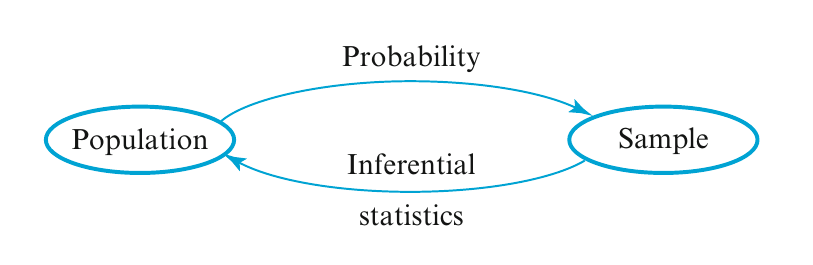
\includegraphics{images/probstat.png}
\caption{}
\end{figure}

Before we can understand what a particular sample can tell us about the
population, we should first understand the uncertainty associated with
taking a sample from a given population. This is why we study
probability before statistics.

\BeginKnitrBlock{example}[Use of manual lap belts in cars equipped with automatic shoulder belt systems]
\protect\hypertarget{exm:unnamed-chunk-9}{}{\label{exm:unnamed-chunk-9}
\iffalse (Use of manual lap belts in cars equipped with automatic
shoulder belt systems) \fi{} }\emph{Probability}: assume that 50\% of
all drivers in a certain metropolitan area regularly use their lap belt
\(\rightarrow\) an assumption about the population. We might ask - How
likely is it that a sample of 100 such drivers will include at least 70
who regularly use their lap belt? - How many of the drivers in a sample
of size 100 can we expect to regularly use their lap belt?

\emph{Inference}: a sample of 100 drivers of such cars revealed that 65
regularly use their lap belt. We might ask\\
- Does this provide substantial evidence for concluding that more than
50\% of all such drivers in this area regularly use their lap belt We
are attempting to use sample information to answer a question about the
structure of the entire population from which the sample was selected.
\EndKnitrBlock{example}

\section{Pictorial and Tabular Methods in Descriptive
Statistics}\label{pictorial-and-tabular-methods-in-descriptive-statistics}

\section{Measures of Location}\label{measures-of-location}

\section{Measures of Variability}\label{measures-of-variability}

\hypertarget{probability}{\chapter{Probability}\label{probability}}

\section*{\texorpdfstring{Introduction\footnote{Reproduced with
  permission from \url{http://www.math.mcgill.ca/dstephens/}}}{Introduction}}\label{introduction1}
\addcontentsline{toc}{section}{Introduction}

The random variation associated with \emph{measurement} procedures in a
scientific analysis requires a framework in which the
\textbf{uncertainty} and \textbf{variability} that are inherent in the
procedure can be handled. The key goal of Probability and Statistical
modelling is to establish a mathematical framework within which
\emph{random} variation (due, for example, to experimental error or
natural variation) can be quantified so that \emph{systematic} variation
(arising due to potentially important biological differences) can be
studied.

Broadly, the \textit{Scientific Process} involves several different
stages:

\begin{equation*}
\begin{array}{cl}
\text{{THEORETICAL MODELLING}} & \rightarrow \text{{MATHEMATICAL/PROBABILISTIC MODELLING}} \\
\downarrow &  \\
\text{{PREDICTION}} &  \\
\downarrow &  \\
\text{{EXPERIMENTATION/OBSERVATION}} &  \\
\downarrow &  \\
\text{{VALIDATION}} &
\end{array}
\end{equation*}

\emph{Mathematical/Probabilistic} \emph{modelling} facilitates
PREDICTION; \emph{Statistical Analysis} provides the means of validation
of predicted behaviour.

To explain the variation in observed data, we need to introduce the
concept of a \emph{probability distribution}. Essentially we need to be
able to model, or specify, or compute the \emph{chance} of observing the
data that we collect or expect to collect. This will then allow us to
assess how likely the data were to occur by chance alone, that is, how
\emph{surprising} the observed data are in light of an assumed
theoretical model.

For example, consider two nucleotide sequences of the same length that
we wish to assess for similarity:

\BeginKnitrBlock{example}[Two nucleotide sequences]
\protect\hypertarget{exm:unnamed-chunk-11}{}{\label{exm:unnamed-chunk-11}
\iffalse (Two nucleotide sequences) \fi{} }

\begin{equation*}
\begin{array}{ll}
\text{{Sequence 1}}{\qquad } & ATAGTAGATACGCACCGAGGA \\
&  \\
\text{{Sequence 2}}{\qquad } & ATCTTAGATAGGCACTGAGGA
\end{array}
\end{equation*}

How can we assess sequence similarity formally ? The number of
discordant positions is 4, but how informative is that summary measure ?
Perhaps we need to assess the chance, for example, that a point mutation
\[ A\rightarrow C \] occurs (as in the discordant position 3) in unit
evolutionary time. Perhaps the chance of observing a sub-sequence

\begin{equation*}
ATCTTA
\end{equation*}

rather than

\begin{equation*}
ATAGTA
\end{equation*}

(in positions 1-6) is important.

\begin{itemize}
\tightlist
\item
  Is the hidden (or \emph{latent}) structure in the sequence,
  corresponding to whether the sequence originates from a coding region
  or otherwise, important ?
\item
  Can we even infer the hidden structure in light of the data we have
  observed ?\\
\end{itemize}
\EndKnitrBlock{example}

These questions can only really be answered when we have an
understanding of randomness and variation. The framework that we will
use to pose and answer such questions formally is given to us by
\emph{probability theory}.

\subsection*{\texorpdfstring{Probability: A Measure of
Uncertainty\footnote{\url{http://www.utstat.toronto.edu/mikevans/jeffrosenthal/book.pdf}}}{Probability: A Measure of Uncertainty}}\label{probability-a-measure-of-uncertainty2}
\addcontentsline{toc}{subsection}{Probability: A Measure of Uncertainty}

Often in life we are confronted by our own ignorance. Whether we are
pondering tonight's traffic jam, tomorrow's weather, next week's stock
prices, an upcoming election, or where we left our hat, often we do not
know an outcome with certainty. Instead, we are forced to guess, to
estimate, to hedge our bets.

\begin{quote}
Probability is the science of uncertainty.
\end{quote}

It provides precise mathematical rules for understanding and analyzing
our own ignorance. It does not tell us tomorrow's weather or next week's
stock prices; rather, it gives us a \textbf{framework for working with
our limited knowledge} and for \textbf{making sensible decisions based
on what we do and do not know}.

To say there is a 40\% chance of rain tomorrow is not to know tomorrow's
weather. Rather, it is to \textbf{know what we do not know} about
tomorrow's weather. In this course, we will develop a more precise
understanding of what it means to say there is a 40\% chance of rain
tomorrow. We will learn how to work with ideas of randomness,
probability, expected value, prediction, estimation, etc., in ways that
are sensible and mathematically clear.

\section{Sample Spaces and Events}\label{sample-spaces-and-events}

\subsection{Sample Spaces}\label{sample-spaces}

\BeginKnitrBlock{definition}[Sample Space]
\protect\hypertarget{def:unnamed-chunk-12}{}{\label{def:unnamed-chunk-12}
\iffalse (Sample Space) \fi{} }The sample space \(\Omega\) is the set of
possible outcomes of an experiment. Points \(\omega\) in \(\Omega\) are
called sample outcomes, realizations, or elements.
\EndKnitrBlock{definition}

\BeginKnitrBlock{example}[Coin tossing]
\protect\hypertarget{exm:unnamed-chunk-13}{}{\label{exm:unnamed-chunk-13}
\iffalse (Coin tossing) \fi{}
}\(\Omega = \left\lbrace H, T \right\rbrace\)
\EndKnitrBlock{example}

\BeginKnitrBlock{example}[Dice]
\protect\hypertarget{exm:unnamed-chunk-14}{}{\label{exm:unnamed-chunk-14}
\iffalse (Dice) \fi{}
}\(\Omega = \left\lbrace 1,2,3,4,5,6 \right\rbrace\)
\EndKnitrBlock{example}

\BeginKnitrBlock{example}[Proportions]
\protect\hypertarget{exm:unnamed-chunk-15}{}{\label{exm:unnamed-chunk-15}
\iffalse (Proportions) \fi{}
}\(\Omega = \left\lbrace x : 0 \leq x \leq 1 \right\rbrace\)
\EndKnitrBlock{example}

\BeginKnitrBlock{example}[Time measurement]
\protect\hypertarget{exm:unnamed-chunk-16}{}{\label{exm:unnamed-chunk-16}
\iffalse (Time measurement) \fi{}
}\(\Omega = \left\lbrace x : x > 0 \right\rbrace = {\mathbb{R}}^{+}\)
\EndKnitrBlock{example}

\BeginKnitrBlock{example}[Temperature measurement]
\protect\hypertarget{exm:unnamed-chunk-17}{}{\label{exm:unnamed-chunk-17}
\iffalse (Temperature measurement) \fi{}
}\(\Omega = \left\{ x:a\leq x\leq b\right\} \subseteq { \mathbb{R}}\)
\EndKnitrBlock{example}

\BeginKnitrBlock{example}[Biological Sequence Analysis]
\protect\hypertarget{exm:unnamed-chunk-18}{}{\label{exm:unnamed-chunk-18}
\iffalse (Biological Sequence Analysis) \fi{} }The experiment may
involve the observation of a nucleotide or protein sequence, so that the
sample space \(\Omega\) may comprise all sequences (of bases/amino
acids) up to a given length, and a sample outcome would be a particular
observed sequence.
\EndKnitrBlock{example}

There are two basic types of experiment: - Counting - Measurement

We shall see that these two types lead to two distinct ways of
specifying probability distributions.

The collection of sample outcomes is a \textbf{set} (a collection of
items) written as

\begin{equation*}
s\in \Omega
\end{equation*}

if \(s\) \emph{is a member of the set} \(\Omega\).

\subsection{Events}\label{events}

\BeginKnitrBlock{definition}[Event]
\protect\hypertarget{def:unnamed-chunk-19}{}{\label{def:unnamed-chunk-19}
\iffalse (Event) \fi{} }An event \(E\) is a subset of the sample space
\(\Omega\) (\(E \subseteq \Omega\)). Events are usually denoted by upper
case letters near the beginning of the alphabet, like \(A, B, C\). An
event which consists of only one outcome is called a simple (or
elementary event); otherwise it is a compound event.
\EndKnitrBlock{definition}

\BeginKnitrBlock{rmdnote}
The sets \(\Omega\) and \(E\) can be either be written as a list of
items, for example,

\begin{equation*}
E=\left\{ s_{1},s_{2},...,s_{n},...\right\}
\end{equation*}

which may a finite or infinite list, or can only be represented by a
continuum of outcomes, for example

\begin{equation*}
E=\left\{ x:0.6<x\leq 2.3\right\}
\end{equation*}
\EndKnitrBlock{rmdnote}

Events are manipulated using \textbf{set theory} notation; if \(A\) and
\(B\) are two events, \(A, B \subseteq \Omega\), then

\begin{itemize}
\tightlist
\item
  \(A \cup B\) is the set of outcomes that belong to \(A\) \textbf{or}
  to \(B\), or to both,
\item
  \(A \cap B\) is the set of outcomes that belong to both \(A\)
  \textbf{and} to \(B\).
\item
  \(A^c\) (complement of \(A\)) is the set of outcomes \textbf{not} in
  \(A\)
\item
  \(A \backslash B = A \cap B^c\)
\end{itemize}

The empty event will be denoted by \(\varnothing\). Two events \(A\) and
\(B\) are mutually exclusive if \(A \cap B = \varnothing\), i.e., the
collection of sample outcomes have no element in common.

\begin{figure}
\centering
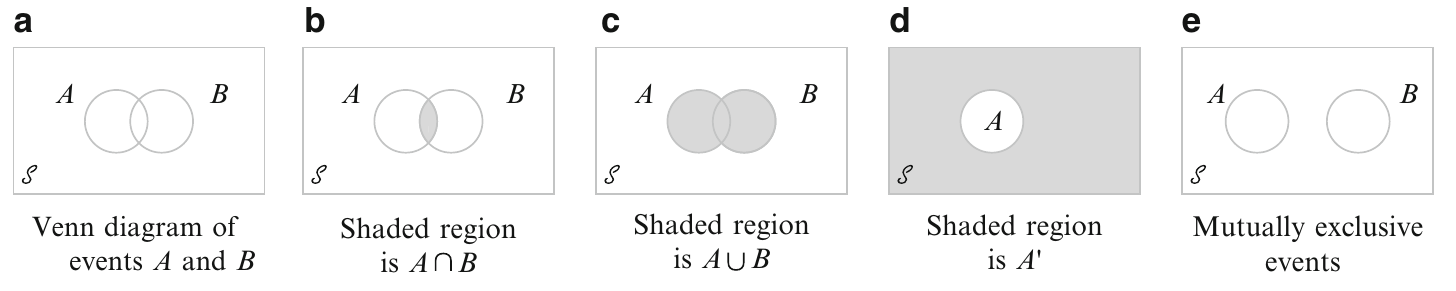
\includegraphics{images/venn.png}
\caption{}
\end{figure}

\section{Axioms, Interpretations, and Properties of
Probability}\label{axioms-interpretations-and-properties-of-probability}

\BeginKnitrBlock{definition}[Axioms (basic properties) of Probability]
\protect\hypertarget{def:unnamed-chunk-21}{}{\label{def:unnamed-chunk-21}
\iffalse (Axioms (basic properties) of Probability) \fi{} }To ensure
that the probability assignments will be consistent with our intuitive
notions of probability, all assign- ments should satisfy the following
axioms (basic properties) of probability

\begin{itemize}
\tightlist
\item
  \textbf{AXIOM 1:} For any event \(A\), \[ P(A) \geq 0 \]
\item
  \textbf{AXIOM 2:} \[ P(\Omega) = 1 \]
\item
  \textbf{AXIOM 3:} If \(A_1, A_2, \ldots\) is an infinite collection of
  disjoint events, then
  \[   P\left(A_1 \cup A_2 \cup \cdots \right) = \sum_{i=1}^{\infty} P(A_i)  \]
\end{itemize}
\EndKnitrBlock{definition}

\BeginKnitrBlock{proposition}
\protect\hypertarget{prp:unnamed-chunk-22}{}{\label{prp:unnamed-chunk-22}
}\(P(\varnothing) = 0\) where \(\varnothing\) is the null event. This in
turn implies that the property contained in Axiom 3 is valid for a
finite collection of events.
\EndKnitrBlock{proposition}

\BeginKnitrBlock{proposition}
\protect\hypertarget{prp:unnamed-chunk-23}{}{\label{prp:unnamed-chunk-23}
}For any event \(A\),\\
\[ P(A) = 1 - P(A^c) \]
\EndKnitrBlock{proposition}

\BeginKnitrBlock{proposition}
\protect\hypertarget{prp:unnamed-chunk-24}{}{\label{prp:unnamed-chunk-24}
}For any event \(A\),\\
\[ P(A) \leq 1 \]
\EndKnitrBlock{proposition}

\BeginKnitrBlock{proposition}
\protect\hypertarget{prp:unnamed-chunk-25}{}{\label{prp:unnamed-chunk-25}
}For any events \(A\) and \(B\),\\
\[ P(A \cup B) = P(A) + P(B) - P(A \cap B) \]
\EndKnitrBlock{proposition}

\section{Counting Techniques}\label{counting-techniques}

When the various outcomes of an experiment are equally likely (the same
probability is assigned to each simple event), the task of computing
probabilities reduces to counting. In particular, if \(N\) is the number
of outcomes in a sample space and \(N(A)\) is the number of outcomes
contained in an event \(A\), then \[ P(A) = \frac{N(A)}{N} \]

\BeginKnitrBlock{proposition}[Product rule for ordered pairs]
\protect\hypertarget{prp:unnamed-chunk-26}{}{\label{prp:unnamed-chunk-26}
\iffalse (Product rule for ordered pairs) \fi{} }If the first element or
object of an ordered pair can be selected in \(n_1\) ways, and for each
of these \(n_1\) ways the second element of the pair can be selected in
\(n_2\) ways, then the number of pairs is \(n_1 \cdot n_2\).
\EndKnitrBlock{proposition}

\subsection{Permutations}\label{permutations}

\BeginKnitrBlock{definition}[Permutation]
\protect\hypertarget{def:unnamed-chunk-27}{}{\label{def:unnamed-chunk-27}
\iffalse (Permutation) \fi{} }Any ordered sequence of \(k\) objects
taken from a set of \(n\) distinct objects is called a permutation of
size \(k\) of the objects. The number of permutations of size \(k\) that
can be constructed from the \(n\) objects is denoted by \(P_k^n\):

\[ P_k^n = \frac{n!}{(n-k)!} \]
\EndKnitrBlock{definition}

\subsection{Combinations}\label{combinations}

\BeginKnitrBlock{definition}[Combination]
\protect\hypertarget{def:unnamed-chunk-28}{}{\label{def:unnamed-chunk-28}
\iffalse (Combination) \fi{} }Given a set of \(n\) distinct objects, any
unordered subset of size \(k\) of the objects is called a combination.
The number of combinations \(n\) of size \(k\) that can be formed from
\(n\) distinct objects will be denoted by

\[ \binom{n}{k} = \frac{n!}{k!(n-k)!} = \frac{P_k^n}{k!} \]
\EndKnitrBlock{definition}

\section{Conditional Probability}\label{conditional-probability}

Conditional probability is the means by which probabilities are updated
in the light of new information. We examine how the information \emph{an
event B has occurred} affects the probability assigned to \(A\).

\BeginKnitrBlock{example}[Flipping Coins]
\protect\hypertarget{exm:flipcoins}{}{\label{exm:flipcoins}
\iffalse (Flipping Coins) \fi{} }We flip three different fair coins,
and\\
\[ \Omega = {H H H, H H T, H T H, H T T, T H H, T H T, T T H, T T T } \]
with \(P(s) = 1/8\) for each \(s \in \Omega\). What is the probability
that the first coin comes up heads?

\[ P(\textrm{first coin heads}) = P({H H H, H H T, H T H, H T T }) = 4/8 = 1/2 \]

But suppose now that an informant tells us that exactly two of the three
coins came up heads. Now what is the probability that the first coin was
heads? if we know that exactly two of the coins were heads, then we know
that the outcome was one of \({H H T , H T H, T H H}\).

Because those three outcomes should (in this case) still all be equally
likely, and because only the first two correspond to the first coin
being heads, we conclude the following: If we know that exactly two of
the three coins are heads, then the probability that the first coin is
heads is \(2/3\).

More precisely, we have computed a conditional probability. That is, we
have determined that, conditional on knowing that exactly two coins came
up heads, the conditional probability of the first coin being heads is
2/3. We write this in mathematical notation as

\[ P(\textrm{first coin heads} | \textrm{two coins heads}) = 2/3. \]

Here the vertical bar \textbar{} stands for \emph{conditional on} or
\emph{given that}.
\EndKnitrBlock{example}

\BeginKnitrBlock{example}[Assembly Lines]
\protect\hypertarget{exm:assembly}{}{\label{exm:assembly} \iffalse (Assembly
Lines) \fi{} }Complex components are assembled in a plant that uses two
different assembly lines, \(A\) and \(A^c\) . Line \(A\) uses older
equipment than \(A^c\), so it is somewhat slower and less reliable.
\(B\) are the defective components and \(B^c\) are the nondefective.

\begin{longtable}[]{@{}lll@{}}
\toprule
& Condition &\tabularnewline
\midrule
\endhead
\textbf{Line} & \(B\) & \(B^c\)\tabularnewline
\(A\) & 2 & 6\tabularnewline
\(A^c\) & 1 & 9\tabularnewline
\bottomrule
\end{longtable}

The sales manager randomly selects 1 of these 18 components for a
demonstration\\
\[ P(\textrm{line A component was selected}) = P(A) = \frac{N(A)}{N} = \frac{8}{18} = 0.444 \]

However, if the chosen component turns out to be defective, then the
event \(B\) has occurred, so the component must have been 1 of the 3 in
the \(B\) column of the table. Since these 3 components are equally
likely among themselves after \(B\) has occurred

\[ P(\textrm{line A component was selected} | \textrm{Defective}) = \frac{2}{3} = \frac{2/18}{3/18} = \frac{P(A \cap B)}{P(B)} \]
\EndKnitrBlock{example}

In Example \ref{exm:assembly}, the conditional probability is expressed
as a ratio of \textbf{unconditional probabilities}. The numerator is the
probability of the intersection of the two events, whereas the
denominator is the probability of the conditioning event \(B\). Given
that \(B\) has occurred, the relevant sample space is no longer
\(\Omega\) but consists of just outcomes in \(B\); A has occurred if and
only if \emph{one of the outcomes in the intersection} occurred, so the
conditional probability of A given B is proportional to \(P(A \cap B)\).
The proportionality constant \(1/P(B)\) is used to ensure that the
probability \(P(B | B)\) of the new sample space \(B\) equals 1.

\BeginKnitrBlock{definition}[Conditional Probability]
\protect\hypertarget{def:condprob}{}{\label{def:condprob}
\iffalse (Conditional Probability) \fi{} }Given two events \(A\) and
\(B\), with \(P(B) > 0\), the conditional probability of \(A\) given
\(B\) is equal to

\[ P(A|B) = \frac{P(A \cap B)}{P(B)}  \]
\EndKnitrBlock{definition}

In example \ref{exm:flipcoins}, let\\
- \(A = {H H H, H H T, H T H, H T T }\) be the event that the first coin
is heads\\
- \(B = {H H T, H T H, T H H}\) be the event that exactly two coins were
heads

It follows that

\[ A \cap B = {H H T, H T H}\]

Therefore

\[ P(A|B) = \frac{P(A \cap B)}{P(B)} = \frac{P({H H T, H T H})}{P({H H T, H T H, T H H})} = \frac{2/8}{3/8} = \frac{2}{3}\]

\BeginKnitrBlock{example}[Balanced die]
\protect\hypertarget{exm:unnamed-chunk-29}{}{\label{exm:unnamed-chunk-29}
\iffalse (Balanced die) \fi{} }Suppose a balanced die is tossed in the
next room. We are told that a number less than 4 was observed. What is
the probability the number was either 1 or 2?
\EndKnitrBlock{example}

\BeginKnitrBlock{example}[Two Balanced Dice v1]
\protect\hypertarget{exm:unnamed-chunk-30}{}{\label{exm:unnamed-chunk-30}
\iffalse (Two Balanced Dice v1) \fi{} }Toss two balanced dice. Let \(A\)
= \{sum of 5\} and \(B\) = \{first die is \(\leq\) 2\}. Find \(P(A|B)\)
\EndKnitrBlock{example}

\BeginKnitrBlock{example}[Two Balanced Dice v2]
\protect\hypertarget{exm:unnamed-chunk-31}{}{\label{exm:unnamed-chunk-31}
\iffalse (Two Balanced Dice v2) \fi{} }Two balanced dice are tossed.
What is the probability that the first die gives a number less than
three, given that the sum is odd?
\EndKnitrBlock{example}

\BeginKnitrBlock{example}[Unbalanced Die]
\protect\hypertarget{exm:unbalanced}{}{\label{exm:unbalanced}
\iffalse (Unbalanced Die) \fi{} }Toss an unbalanced die with probs
\(P(1)=.1\), \(P(2)=.1\), \(P(3)=.3\), \(P(4)=.2\), \(P(5)=.1\),
\(P(6)=.2\). Let \(A={\geq 5}\) and \(B={\geq 2}\). Find \(P(A|B)\).
\EndKnitrBlock{example}

\BeginKnitrBlock{example}[Two Balanced Coins]
\protect\hypertarget{exm:unnamed-chunk-32}{}{\label{exm:unnamed-chunk-32}
\iffalse (Two Balanced Coins) \fi{} }Two balanced coins were tossed, and
it is known that at least one was a head. What is the probability that
both were heads?
\EndKnitrBlock{example}

\BeginKnitrBlock{example}[Two Cards]
\protect\hypertarget{exm:unnamed-chunk-33}{}{\label{exm:unnamed-chunk-33}
\iffalse (Two Cards) \fi{} }Two cards are drawn without replacement from
a standard deck. Find the probability that

\begin{enumerate}
\def\labelenumi{\arabic{enumi})}
\tightlist
\item
  the second is an ace, given that the first is not an ace.\\
\item
  the second is an ace.\\
\item
  the first was an ace, given that the second is an ace.
\end{enumerate}
\EndKnitrBlock{example}

\BeginKnitrBlock{example}[Numbers in a Hat]
\protect\hypertarget{exm:unnamed-chunk-34}{}{\label{exm:unnamed-chunk-34}
\iffalse (Numbers in a Hat) \fi{} }The numbers 1 to 5 are written on
five slips of paper and placed in a hat. Two slips are drawn at random
without replacement. What is the probability that the first number is 3,
given a sum of seven?
\EndKnitrBlock{example}

\BeginKnitrBlock{example}[One Card]
\protect\hypertarget{exm:unnamed-chunk-35}{}{\label{exm:unnamed-chunk-35}
\iffalse (One Card) \fi{} }A card is selected at random (i.e.~every card
has the same probability of being chosen) from a deck of 52. What is the
probability it is a red card or a face card?
\EndKnitrBlock{example}

Definition \ref{def:condprob} immediately leads to the
\emph{multiplication formula}

\BeginKnitrBlock{definition}[Multiplicative Rule]
\protect\hypertarget{def:multformula}{}{\label{def:multformula}
\iffalse (Multiplicative Rule) \fi{} }\[P(A \cap B) = P(A|B) P(B)\]

and

\[P(A \cap B) = P(B|A) P(A)\]
\EndKnitrBlock{definition}

This allows us to compute the joint probability of \(A\) and \(B\) when
we are given the probability of \(B\) and the conditional probability of
\(A\) given \(B\), and vice versa.

\BeginKnitrBlock{example}[Fish in a Tank]
\protect\hypertarget{exm:unnamed-chunk-36}{}{\label{exm:unnamed-chunk-36}
\iffalse (Fish in a Tank) \fi{} }A tank has three red fish and two blue
fish. Two fish are chosen at random and without replacement. What is the
probability of getting

\begin{enumerate}
\def\labelenumi{\arabic{enumi})}
\tightlist
\item
  red fish first and then a blue fish?\\
\item
  both fish red?\\
\item
  one red fish and one blue fish?
\end{enumerate}
\EndKnitrBlock{example}

\subsection{Law of Total Probability}\label{law-of-total-probability}

Recall that events \(A_1, A_2, \ldots, A_k\) are mutually exclusive if
no two have any common outcomes. The events are exhaustive if one
\(A_i\) must occure, so that\\
\[A_1 \cup A_2 \cup \cdots \cup A_k = \Omega \]

\BeginKnitrBlock{theorem}[Law of Total Probability]
\protect\hypertarget{thm:totprob}{}{\label{thm:totprob} \iffalse (Law of
Total Probability) \fi{} }Let \(A_1, A_2, \ldots, A_k\) be mutually
exclusive and exhaustive events. Then for any other event \(B\),\\
\[P(B) = P(B|A_1) P(A_1) + \cdots + P(B|A_k)P(A_k) = \sum_{i=1}^{k} P(B|A_i) P(A_i)\]
\EndKnitrBlock{theorem}

\textbf{Proof}: Because the \(A_i\)'s are mutually exclusive and
exhaustive, if \(B\) occurs it must be in conjunction with exactly one
of the \(A_i\)'s. That is, \(B= (A_1\textrm{ and }B)\) or \(\ldots\) or
\((A_k\textrm{ and }B)\) which is equal to
\((A_1 \cap B) \cup \cdots \cup (A_k \cap B)\), where the events
\((A_i \cap B)\) are mutually exclusive.

\begin{figure}
\centering
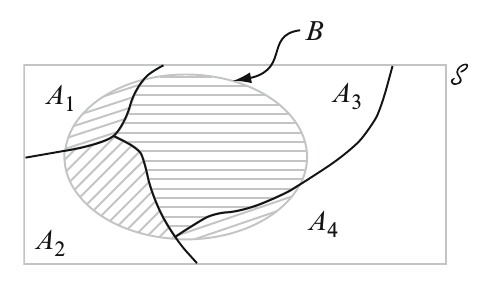
\includegraphics{images/totalprob.png}
\caption{}
\end{figure}

Thus we have

\[P(B) =\sum_{i=1}^{k} P(A_i \cap B) = \sum_{i=1}^{k} P(B|A_i) P(A_i) \]

\BeginKnitrBlock{example}[Long Hair]
\protect\hypertarget{exm:unnamed-chunk-37}{}{\label{exm:unnamed-chunk-37}
\iffalse (Long Hair) \fi{} }Suppose a class contains 60\% girls and 40\%
boys. Suppose that 30\% of the girls have long hair, and 20\% of the
boys have long hair. A student is chosen uniformly at random from the
class. What is the probability that the chosen student will have long
hair?
\EndKnitrBlock{example}

\subsection{Bayes' Rule}\label{bayes-rule}

\BeginKnitrBlock{theorem}[Bayes' Rule]
\protect\hypertarget{thm:bayesdef}{}{\label{thm:bayesdef} \iffalse (Bayes'
Rule) \fi{} }Let \(A_1, \ldots, A_k\) be a collection of mutually
exclusive and exhaustive events with \(P(A_i) > 0\) for
\(i=1, \ldots, k\). Then for any other event B, for which \(P(B)>0\), we
have

\[ P(A_j | B) = \frac{P(A_j \cap B)}{P(B)} = \frac{P(B|A_j) P(A_j)}{\sum_{i=1}^k P(B|A_i) P(A_i)}, \quad j=1, \ldots, k   \]
\EndKnitrBlock{theorem}

The transition from the second to the third expression in Theorem
\ref{thm:bayesdef} rests on using the multiplication rule in the
numerator and the law of total probability in the denominator.

\BeginKnitrBlock{example}[Urns]
\protect\hypertarget{exm:unnamed-chunk-38}{}{\label{exm:unnamed-chunk-38}
\iffalse (Urns) \fi{} }Suppose urn \#1 has 3 red and 2 blue balls, and
urn \#2 has 4 red and 7 blue balls. Suppose one of the two urns is
selected with probability \(1/2\) each, and then one of the balls within
that urn is picked uniformly at random.

\begin{enumerate}
\def\labelenumi{\arabic{enumi})}
\tightlist
\item
  What is the probability that urn \#2 is selected at the first stage
  (event A) and a blue ball is selected at the second stage (event B)?\\
\item
  Compute the probability that a blue ball is obtained.\\
\item
  Now suppose we are given the information that the ball picked is blue.
  What is probability that we had selected urn \#2?
\end{enumerate}
\EndKnitrBlock{example}

\BeginKnitrBlock{example}[Large Bridges]
\protect\hypertarget{exm:unnamed-chunk-39}{}{\label{exm:unnamed-chunk-39}
\iffalse (Large Bridges) \fi{} }There are three Canadian firms which
build large bridges, firm 1, firm 2, and firm 3. 20\% of Canadian large
bridges have been built by firm 1, 30\% by firm 2, and the rest by firm
3. 5\% of the bridges built by firm 1 have collapsed, while 10\% of
those by firm 2 have collapsed, and 30\% by firm 3 have collapsed.

\begin{enumerate}
\def\labelenumi{\arabic{enumi})}
\tightlist
\item
  What is the probability that a bridge collapses?\\
\item
  Suppose it is reported in tomorrow's newspaper that a large bridge has
  collapsed. What is the probability it was built by firm 1?
\end{enumerate}
\EndKnitrBlock{example}

\section{Independence}\label{independence}

If we flip a fair coin twice, then the probability of two heads is
\(1/2 \times 1/2\). We multiply the probabilities because we regard the
two tosses as independent. The formal definition of independence is as
follows:

\BeginKnitrBlock{definition}[Indepent Events]
\protect\hypertarget{def:indep}{}{\label{def:indep} \iffalse (Indepent
Events) \fi{} }Two events \(A\) and \(B\) are independent if\\
\[ P(A \cap B) = P(A) P(B) \]
\EndKnitrBlock{definition}

Now, because \(P(A | B) = P( A \cap B)/P(B)\), we see that \(A\) and
\(B\) are independent if and only if \(P(A | B) = P(A)\) or
\(P(B | A) = P(B)\), provided that \(P(A) > 0\) and \(P(B) > 0\).
Definition \ref{def:indep} has the advantage that it remains valid even
if \(P(B) = 0\) or \(P(A) = 0\), respectively. Intuitively, events \(A\)
and \(B\) are independent if neither one has any impact on the
probability of the other.

\BeginKnitrBlock{example}[Toss a fair coin 10 times]
\protect\hypertarget{exm:unnamed-chunk-40}{}{\label{exm:unnamed-chunk-40}
\iffalse (Toss a fair coin 10 times) \fi{} }Toss a fair coin 10 times.
Let \(A = {\textrm{at least one head}}\). Let \(T_j\) be the event that
tails occurs on the \(j^{th}\) toss. Find \(P(A)\)
\EndKnitrBlock{example}

\BeginKnitrBlock{example}[Unbalance Die Revisited]
\protect\hypertarget{exm:unnamed-chunk-41}{}{\label{exm:unnamed-chunk-41}
\iffalse (Unbalance Die Revisited) \fi{} }In Example
\ref{exm:unbalanced}, if \(A\) is the event that the die was 5, and
\(B\) is the event that the coin was tails, then calculate
\(P(A), P(B)\) and \(P(A\cap B)\)
\EndKnitrBlock{example}

\chapter{Discrete Random Variables and Probability
Distributions}\label{discrete-random-variables-and-probability-distributions}

\section*{Introduction}\label{introduction}
\addcontentsline{toc}{section}{Introduction}

In Chapter \protect\hyperlink{probability}{2}, we discussed the
probability model as the central object of study in the theory of
probability. This required defining a probability measure \(P\) on a
class of subsets of the sample space \(\Omega\). For example, for an
experiment with possible sample outcomes denoted by the
\emph{sample space} \(\Omega\), an \emph{event} \(E\) was defined as any
collection of sample outcomes, that is, any subset of the set
\(\Omega\).

\[
\begin{array}{ccll}
\text{EXPERIMENT} & \longrightarrow \text{SAMPLE OUTCOMES} & \longrightarrow
\text{EVENTS} & \longrightarrow \text{PROBABILITIES} \\
& \Omega=\left\{ s_{1},s_{2},...\right\} & \longrightarrow E\subseteq S &
\longrightarrow P(E)
\end{array}
\]

In this framework, it is necessary to consider each experiment with its
associated sample space separately - the nature of sample space
\(\Omega\) is typically different for different experiments.

\BeginKnitrBlock{example}[Rainy days]
\protect\hypertarget{exm:unnamed-chunk-43}{}{\label{exm:unnamed-chunk-43}
\iffalse (Rainy days) \fi{} }Count the number of days in February which
have zero precipitation.

\[ \Omega = \left\{ 0,1,2,\ldots,28\right\} \]

Let \(E_{i}\) = \(i\) days have zero precipitation.
\(E_{0},\ldots,E_{28}\) partition \(\Omega\).
\EndKnitrBlock{example}

\BeginKnitrBlock{example}[Footbal Match]
\protect\hypertarget{exm:unnamed-chunk-44}{}{\label{exm:unnamed-chunk-44}
\iffalse (Footbal Match) \fi{} }Count the number of goals in a football
match.

\[ \Omega = \left\{ 0,1,2,3,\ldots \right\} \]

Let \(E_{i}\) = \(i\) goals in the match. \(E_{0},E_{1},E_{2},\ldots\)
partition \(\Omega\)\\
\EndKnitrBlock{example}

\BeginKnitrBlock{rmdnote}
In both of these examples, we need a formula to specify each

\[ P(E_{i}) = p_{i} \]
\EndKnitrBlock{rmdnote}

\BeginKnitrBlock{example}[Operating Temperature]
\protect\hypertarget{exm:unnamed-chunk-46}{}{\label{exm:unnamed-chunk-46}
\iffalse (Operating Temperature) \fi{} }Measure the operating
temperature of an experimental process.

\[ \Omega = \left\{ x: x > T_{min} \right\} \]
\EndKnitrBlock{example}

Here it is difficult to express

\[ P(``\textrm{Measurement is }x") \]

but possible to think about

\[ P (``\textrm{Measurement is }\leq x")=F(x) \]

and now we seek a formula for \(F(x)\) which is a simpler way of
presenting a particular probability assignment.

This chapter is concerned with the definitions of random variables,
distribution functions \(F(x)\), probability/density functions \(f(x)\),
and the development of the concepts necessary for carrying out
calculations for a probability model using these entities
\citep{evans2004probability}.

The concept of a random variable allows us to pass from the experimental
outcomes themselves to a numerical function of the outcomes. There are
two fundamentally different types of random variables
\citep{devore2011modern}:

\begin{enumerate}
\def\labelenumi{\roman{enumi})}
\tightlist
\item
  discrete random variables\\
\item
  continuous random variables
\end{enumerate}

In this chapter, we examine the basic properties and discuss the most
important examples of \textbf{discrete} variables. Chapter
\protect\hyperlink{continuous-variables-and-probability-distributions}{4}
focuses on continuous random variables.

\section{Random Variables}\label{random-variables}

A general notation useful for all such examples can be obtained by
considering a sample space that is \textbf{equivalent} to \(\Omega\) for
a general experiment, but whose form is more familiar.

\BeginKnitrBlock{definition}[Random Variable]
\protect\hypertarget{def:rv}{}{\label{def:rv} \iffalse (Random Variable)
\fi{} }A random variable \(X\) on \(\Omega\) is a function from the
sample space \(\Omega\) to the set \(\mathbb{R}\) of all real numbers
denoted by

\[ X : \Omega \rightarrow \mathbb{R}  \]

Let \(R_X\) denote the range of \(X\).
\EndKnitrBlock{definition}

\(X\) is called a \emph{discrete} random variable if \(R_X\) is a
countable set.

\begin{figure}
\centering
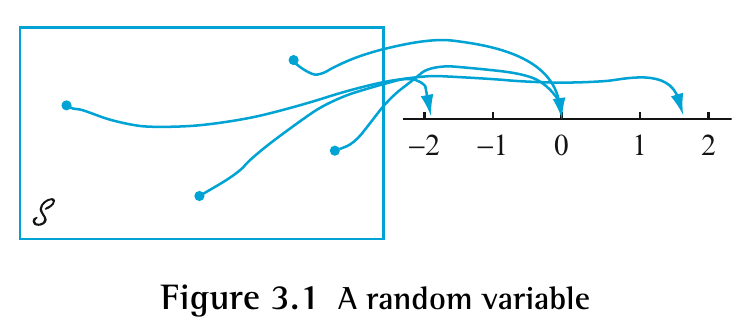
\includegraphics{images/rv.png}
\caption{}
\end{figure}

\BeginKnitrBlock{rmdnote}
Random variables are customarily denoted by uppercase letters, such as
\(X\) and \(Y\), lowercase letters to represent some particular value of
the corresponding random variable. The notation \(X(s) = x\) means that
\(x\) is the value associated with the outcome \(s\) by the rv \(X\).
\EndKnitrBlock{rmdnote}

\BeginKnitrBlock{example}[Coin Toss]
\protect\hypertarget{exm:unnamed-chunk-48}{}{\label{exm:unnamed-chunk-48}
\iffalse (Coin Toss) \fi{} }Suppose a coin is tossed three times. Let
\(X\) be the number of heads observed. The sample space is

\[ \Omega = \left\lbrace \underbrace{HHT}_{3},\underbrace{HHT}_{2},\underbrace{HTH}_{2},\underbrace{HTT}_{1}, \underbrace{THH}_{2}, \underbrace{THT}_{1}, \underbrace{TTH}_{1}, \underbrace{TTT}_{0} \right\rbrace   \]

That is, we have \(X(HHH) = 3\), \(X(HHT) = 2\), \(X(HTH) = 2\), and so
on. Hence \(R_X = \left\lbrace 0,1,2,3 \right\rbrace\)
\EndKnitrBlock{example}

\BeginKnitrBlock{example}[A Very Simple Random Variable]
\protect\hypertarget{exm:simple}{}{\label{exm:simple} \iffalse (A Very
Simple Random Variable) \fi{} }Let the random variable
\(X: \left\lbrace \textrm{rain, snow, clear} \right\rbrace \rightarrow \mathbb{R}\)
by \(X(rain) = 3\), \(X(snow) = 6\), and \(X(clear) = -2.7\).
\EndKnitrBlock{example}

We now present several further examples. The point is, we can define
random variables any way we like, as long as they are functions from the
sample space to \(\mathbb{R}\).

\BeginKnitrBlock{example}[A Very Simple Random Variable 2]
\protect\hypertarget{exm:unnamed-chunk-49}{}{\label{exm:unnamed-chunk-49}
\iffalse (A Very Simple Random Variable 2) \fi{} }For the case
\(\Omega = \left\lbrace \textrm{rain, snow, clear} \right\rbrace\), we
might define a second random variable \(Y\) by saying that \(Y = 0\) if
it rains, \(Y = -1/2\) if it snows, and \(Y = 7/8\) if it is clear. That
is \(Y(rain) = 0\), \(Y(snow) = 1/2\), and \(Y(rain) = 7/8\).
\EndKnitrBlock{example}

\BeginKnitrBlock{example}[A Very Simple Random Variable 3]
\protect\hypertarget{exm:unnamed-chunk-50}{}{\label{exm:unnamed-chunk-50}
\iffalse (A Very Simple Random Variable 3) \fi{} }If the sample space
corresponds to flipping three different coins, then we could let \(X\)
be the total number of heads showing, let \(Y\) be the total number of
tails showing, let \(Z = 0\) if there is exactly one head, and otherwise
\(Z = 17\).
\EndKnitrBlock{example}

\BeginKnitrBlock{example}[Constants as Random Variables]
\protect\hypertarget{exm:unnamed-chunk-51}{}{\label{exm:unnamed-chunk-51}
\iffalse (Constants as Random Variables) \fi{} }As a special case, every
constant value \(c\) is also a random variable, by saying that
\(c(s) = c\) for all \(s \in \Omega\). Thus, 5 is a random variable, as
is 3 or −21.6.
\EndKnitrBlock{example}

\BeginKnitrBlock{example}[Indicator Functions]
\protect\hypertarget{exm:unnamed-chunk-52}{}{\label{exm:unnamed-chunk-52}
\iffalse (Indicator Functions) \fi{} }If \(A\) is any event, then we can
define the indicator function of \(A\), written \(I_A\), to be the
random variable

\[I_A(s)  = \begin{cases} 1 & s \in A \\ 0 & s \notin A   \end{cases} \]
\EndKnitrBlock{example}

Suppose \(X\) is a random variable. We know that different states \(s\)
occur with different probabilities. It follows that \(X(s)\) also takes
different values with different probabilities. These probabilities are
called the \textbf{distribution} of \(X\); we consider them next.

\section{Probability Distributions for Discrete Random
Variables}\label{probability-distributions-for-discrete-random-variables}

Because random variables are defined to be functions of the outcome
\(s\), and because the outcome \(s\) is assumed to be random (i.e., to
take on different values with different probabilities), it follows that
the value of a random variable will itself be random (as the name
implies).

Specifically, if \(X\) is a random variable, then what is the
probability that \(X\) will equal some particular value \(x\)? Well,
\(X = x\) precisely when the outcome \(s\) is chosen such that
\(X(s) = x\).

\section{Expected Values of Discrete Random
Variables}\label{expected-values-of-discrete-random-variables}

\section{Moments and Moment Generating
Functions}\label{moments-and-moment-generating-functions}

\section{The Binomial Probability
Distribution}\label{the-binomial-probability-distribution}

\section{The Poisson Probability
Distribution}\label{the-poisson-probability-distribution}

\hypertarget{continuous-variables-and-probability-distributions}{\chapter{Continuous
Variables and Probability
Distributions}\label{continuous-variables-and-probability-distributions}}

\section*{Introduction}\label{introduction-1}
\addcontentsline{toc}{section}{Introduction}

\appendix


\chapter{Vectorization, *apply and for
loops}\label{vectorization-apply-and-for-loops}

This section will cover the basics of vectorizations, the
\texttt{*apply} family of functions and \texttt{for} loops.

\section{Vectorization}\label{vectorization}

Almost everything in \texttt{R} is a vector. A scalar is really a vector
of length 1 and a \texttt{data.frame} is a collection of vectors. An
nice feature of \texttt{R} is its vectorized capabilities. Vectorization
indicates that a function operates on a whole vector of values at the
same time and not just on a single value\footnote{\url{http://www.dummies.com/how-to/content/how-to-vectorize-your-functions-in-r.html}}.
If you have have ever taken a basic linear algebra course, this concept
will be familiar to you. \newline  \vspace{0.1in} Take for example two
vectors: \newline
\vspace{0.1in} \[
\begin{bmatrix} 1 \\ 2 \\ 3 \end{bmatrix} + 
\begin{bmatrix} 1 \\ 2 \\ 3 \end{bmatrix} =
\begin{bmatrix} 2 \\ 4 \\ 6 \end{bmatrix}
\] \newline  \vspace{0.1in} The corresponding \texttt{R} code is given
by:

\begin{Shaded}
\begin{Highlighting}[]
\NormalTok{a <-}\StringTok{ }\KeywordTok{c}\NormalTok{(}\DecValTok{1}\NormalTok{,}\DecValTok{2}\NormalTok{,}\DecValTok{3}\NormalTok{)}
\NormalTok{b <-}\StringTok{ }\KeywordTok{c}\NormalTok{(}\DecValTok{1}\NormalTok{,}\DecValTok{2}\NormalTok{,}\DecValTok{3}\NormalTok{)}
\NormalTok{a}\OperatorTok{+}\NormalTok{b}
\CommentTok{#> [1] 2 4 6}
\end{Highlighting}
\end{Shaded}

Many of the \texttt{base} functions in \texttt{R} are already
vectorized. Here are some common examples:

\begin{Shaded}
\begin{Highlighting}[]

\CommentTok{# generate a sequence of numbers from 1 to 10}
\NormalTok{(a <-}\StringTok{ }\DecValTok{1}\OperatorTok{:}\DecValTok{10}\NormalTok{)}
\CommentTok{#>  [1]  1  2  3  4  5  6  7  8  9 10}

\CommentTok{# sum the numbers from 1 to 10}
\KeywordTok{sum}\NormalTok{(a)}
\CommentTok{#> [1] 55}

\CommentTok{# calculate sums of each column}
\KeywordTok{colSums}\NormalTok{(iris[, }\OperatorTok{-}\DecValTok{5}\NormalTok{])}
\CommentTok{#> Sepal.Length  Sepal.Width Petal.Length  Petal.Width }
\CommentTok{#>        876.5        458.6        563.7        179.9}
\end{Highlighting}
\end{Shaded}

\begin{quote}
\textbf{Exercise}: What happens when you sum two vectors of different
lengths?
\end{quote}

\section{\texorpdfstring{Family of \texttt{*apply}
functions}{Family of *apply functions}}\label{family-of-apply-functions}

\begin{itemize}
\tightlist
\item
  \texttt{apply}, \texttt{lapply} and \texttt{sapply} are some of the
  most commonly used class of functions in \texttt{R}
\item
  \texttt{*apply} functions are not necessarily faster than loops, but
  can be easier to read (and vice cersa)
\item
  \texttt{apply} is used when you need to perform an operation on every
  row or column of a matrix or data.frame
\item
  \texttt{lapply} and \texttt{sapply} differ in the format of the
  output. The former returns a list while the ladder returns a vector
\item
  There are other \texttt{*apply} functions such as \texttt{tapply},
  \texttt{vapply} and \texttt{mapply} with similar functionality and
  purpose
\end{itemize}

\subsection{Loops vs.~Apply}\label{loops-vs.apply}

\begin{Shaded}
\begin{Highlighting}[]

\CommentTok{# Getting the row means of two columns}
\CommentTok{# Generate data}
\NormalTok{N <-}\StringTok{ }\DecValTok{10000}
\NormalTok{x1 <-}\StringTok{ }\KeywordTok{runif}\NormalTok{(N)}
\NormalTok{x2 <-}\StringTok{ }\KeywordTok{runif}\NormalTok{(N)}
\NormalTok{d <-}\StringTok{ }\KeywordTok{as.data.frame}\NormalTok{(}\KeywordTok{cbind}\NormalTok{(x1, x2))}
\KeywordTok{head}\NormalTok{(d)}
\CommentTok{#>        x1     x2}
\CommentTok{#> 1 0.57632 0.9615}
\CommentTok{#> 2 0.56474 0.1950}
\CommentTok{#> 3 0.07399 0.3001}
\CommentTok{#> 4 0.45387 0.3823}
\CommentTok{#> 5 0.37328 0.1197}
\CommentTok{#> 6 0.33132 0.9891}

\CommentTok{# Loop:}
\CommentTok{# create a vector to store the results in }
\NormalTok{rowMeanFor <-}\StringTok{ }\KeywordTok{vector}\NormalTok{(}\StringTok{"double"}\NormalTok{, N)}

\ControlFlowTok{for}\NormalTok{ (i }\ControlFlowTok{in} \KeywordTok{seq_len}\NormalTok{(N)) \{}
\NormalTok{        rowMeanFor[[i]] <-}\StringTok{ }\KeywordTok{mean}\NormalTok{(}\KeywordTok{c}\NormalTok{(d[i, }\DecValTok{1}\NormalTok{], d[i, }\DecValTok{2}\NormalTok{]))}
\NormalTok{\}}

\CommentTok{# Apply:}
\NormalTok{rowMeanApply <-}\StringTok{ }\KeywordTok{apply}\NormalTok{(d, }\DecValTok{1}\NormalTok{, mean)}

\CommentTok{# are the results equal}
\KeywordTok{all.equal}\NormalTok{(rowMeanFor,rowMeanApply)}
\CommentTok{#> [1] TRUE}
\end{Highlighting}
\end{Shaded}

\subsection{\texorpdfstring{Descriptive Statistics using
\texttt{*apply}}{Descriptive Statistics using *apply}}\label{descriptive-statistics-using-apply}

\begin{Shaded}
\begin{Highlighting}[]
\KeywordTok{data}\NormalTok{(women)}
\CommentTok{# data structure}
\KeywordTok{str}\NormalTok{(women)}
\CommentTok{#> 'data.frame':    15 obs. of  2 variables:}
\CommentTok{#>  $ height: num  58 59 60 61 62 63 64 65 66 67 ...}
\CommentTok{#>  $ weight: num  115 117 120 123 126 129 132 135 139 142 ...}

\CommentTok{# calculate the mean for each column}
\KeywordTok{apply}\NormalTok{(women, }\DecValTok{2}\NormalTok{, mean)}
\CommentTok{#> height weight }
\CommentTok{#>   65.0  136.7}

\CommentTok{# apply 'fivenum' function to each column}
\KeywordTok{vapply}\NormalTok{(women, fivenum, }\KeywordTok{c}\NormalTok{(}\StringTok{"Min."}\NormalTok{ =}\StringTok{ }\DecValTok{0}\NormalTok{, }\StringTok{"1st Qu."}\NormalTok{ =}\StringTok{ }\DecValTok{0}\NormalTok{, }\StringTok{"Median"}\NormalTok{ =}\StringTok{ }\DecValTok{0}\NormalTok{, }
                         \StringTok{"3rd Qu."}\NormalTok{ =}\StringTok{ }\DecValTok{0}\NormalTok{, }\StringTok{"Max."}\NormalTok{ =}\StringTok{ }\DecValTok{0}\NormalTok{))}
\CommentTok{#>         height weight}
\CommentTok{#> Min.      58.0  115.0}
\CommentTok{#> 1st Qu.   61.5  124.5}
\CommentTok{#> Median    65.0  135.0}
\CommentTok{#> 3rd Qu.   68.5  148.0}
\CommentTok{#> Max.      72.0  164.0}
\end{Highlighting}
\end{Shaded}

\subsection{\texorpdfstring{Creating new columns using
\texttt{sapply}}{Creating new columns using sapply}}\label{creating-new-columns-using-sapply}

You can apply a \emph{user defined function} to columns or the entire
data frame:

\begin{Shaded}
\begin{Highlighting}[]
\CommentTok{# the ouput of sapply is a vector}
\CommentTok{# the 's' in sapply stands for 'simplified' apply}
\NormalTok{mtcars}\OperatorTok{$}\NormalTok{gear2 <-}\StringTok{ }\KeywordTok{sapply}\NormalTok{(mtcars}\OperatorTok{$}\NormalTok{gear, }
                       \ControlFlowTok{function}\NormalTok{(i) }\ControlFlowTok{if}\NormalTok{ (i}\OperatorTok{==}\DecValTok{4}\NormalTok{) }\StringTok{"alot"} \ControlFlowTok{else} \StringTok{"some"}\NormalTok{)}

\KeywordTok{head}\NormalTok{(mtcars)[,}\KeywordTok{c}\NormalTok{(}\StringTok{"gear"}\NormalTok{,}\StringTok{"gear2"}\NormalTok{)]}
\CommentTok{#>                   gear gear2}
\CommentTok{#> Mazda RX4            4  alot}
\CommentTok{#> Mazda RX4 Wag        4  alot}
\CommentTok{#> Datsun 710           4  alot}
\CommentTok{#> Hornet 4 Drive       3  some}
\CommentTok{#> Hornet Sportabout    3  some}
\CommentTok{#> Valiant              3  some}
\end{Highlighting}
\end{Shaded}

\subsection{\texorpdfstring{Applying functions to subsets using
\texttt{tapply}}{Applying functions to subsets using tapply}}\label{applying-functions-to-subsets-using-tapply}

\begin{Shaded}
\begin{Highlighting}[]

\CommentTok{# Fisher's famous dataset }
\KeywordTok{data}\NormalTok{(iris)}
\KeywordTok{str}\NormalTok{(iris)}
\CommentTok{#> 'data.frame':    150 obs. of  5 variables:}
\CommentTok{#>  $ Sepal.Length: num  5.1 4.9 4.7 4.6 5 5.4 4.6 5 4.4 4.9 ...}
\CommentTok{#>  $ Sepal.Width : num  3.5 3 3.2 3.1 3.6 3.9 3.4 3.4 2.9 3.1 ...}
\CommentTok{#>  $ Petal.Length: num  1.4 1.4 1.3 1.5 1.4 1.7 1.4 1.5 1.4 1.5 ...}
\CommentTok{#>  $ Petal.Width : num  0.2 0.2 0.2 0.2 0.2 0.4 0.3 0.2 0.2 0.1 ...}
\CommentTok{#>  $ Species     : Factor w/ 3 levels "setosa","versicolor",..: 1 1 1 1 1 1 1 1 1 1 ...}

\CommentTok{# mean sepal length by species }
\KeywordTok{tapply}\NormalTok{(iris}\OperatorTok{$}\NormalTok{Sepal.Length, iris}\OperatorTok{$}\NormalTok{Species, mean)}
\CommentTok{#>     setosa versicolor  virginica }
\CommentTok{#>      5.006      5.936      6.588}
\end{Highlighting}
\end{Shaded}

\subsection{\texorpdfstring{Nested for loops using
\texttt{mapply}}{Nested for loops using mapply}}\label{nested-for-loops-using-mapply}

\texttt{mapply} is my favorite \texttt{base} \texttt{R} function and
here are some reasons why:

\begin{itemize}
\tightlist
\item
  Using \texttt{mapply} is equivalent to writing nested \texttt{for}
  loops except that it is 100\% more human readable and less prone to
  errors
\item
  It is an effective way of conducting simulations because it iterates
  of many arguments
\end{itemize}

Let's say you want to generate random samples from a normal distribution
with varying means and standard deviations. Of course the brute force
way would be to write out the command once, copy paste as many times as
you want, and then manually change the arguments for \texttt{mean} and
\texttt{sd} in the \texttt{rnorm} function as so:

\begin{Shaded}
\begin{Highlighting}[]
\NormalTok{v1 <-}\StringTok{ }\KeywordTok{rnorm}\NormalTok{(}\DecValTok{100}\NormalTok{, }\DataTypeTok{mean =} \DecValTok{5}\NormalTok{, }\DataTypeTok{sd =} \DecValTok{1}\NormalTok{)}
\NormalTok{v2 <-}\StringTok{ }\KeywordTok{rnorm}\NormalTok{(}\DecValTok{100}\NormalTok{, }\DataTypeTok{mean =} \DecValTok{10}\NormalTok{, }\DataTypeTok{sd =} \DecValTok{5}\NormalTok{)}
\NormalTok{v3 <-}\StringTok{ }\KeywordTok{rnorm}\NormalTok{(}\DecValTok{100}\NormalTok{, }\DataTypeTok{mean =} \OperatorTok{-}\DecValTok{3}\NormalTok{, }\DataTypeTok{sd =} \DecValTok{10}\NormalTok{)}
\end{Highlighting}
\end{Shaded}

This isn't too bad for three vectors. But what if you want to generate
many more combinations of means and sds ? Furthermore, how can you keep
track of the parameters you used? Now lets consider the \texttt{mapply}
function:

\begin{Shaded}
\begin{Highlighting}[]
\NormalTok{means <-}\StringTok{ }\KeywordTok{c}\NormalTok{(}\DecValTok{5}\NormalTok{,}\DecValTok{10}\NormalTok{,}\OperatorTok{-}\DecValTok{3}\NormalTok{) ; sds <-}\StringTok{ }\KeywordTok{c}\NormalTok{(}\DecValTok{1}\NormalTok{,}\DecValTok{5}\NormalTok{,}\DecValTok{10}\NormalTok{) }

\CommentTok{# MoreArgs is a list of arguments that dont change}
\NormalTok{randomNormals <-}\StringTok{ }\KeywordTok{mapply}\NormalTok{(rnorm, }\DataTypeTok{mean =}\NormalTok{ means, }\DataTypeTok{sd =}\NormalTok{ sds, }
                        \DataTypeTok{MoreArgs =} \KeywordTok{list}\NormalTok{(}\DataTypeTok{n =} \DecValTok{100}\NormalTok{))}

\KeywordTok{head}\NormalTok{(randomNormals)}
\CommentTok{#>       [,1]   [,2]    [,3]}
\CommentTok{#> [1,] 3.836  8.771   5.144}
\CommentTok{#> [2,] 4.525  9.376  -2.280}
\CommentTok{#> [3,] 4.072 13.144   2.940}
\CommentTok{#> [4,] 4.737 18.210 -13.118}
\CommentTok{#> [5,] 5.690 22.951  -7.008}
\CommentTok{#> [6,] 4.826  7.615 -15.323}
\end{Highlighting}
\end{Shaded}

The following diagram (from
\href{http://r4ds.had.co.nz/iteration.html\#mapping-over-multiple-arguments}{r4ds})
describes exactly what is going on in the above function call to
\texttt{mapply}:

\begin{figure}
\centering
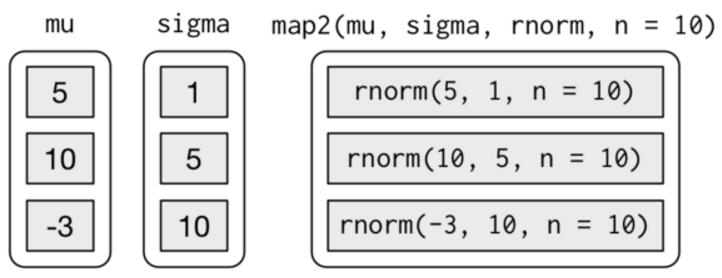
\includegraphics{images/mapply.png}
\caption{}
\end{figure}

Advantages:

\begin{enumerate}
\def\labelenumi{\arabic{enumi}.}
\tightlist
\item
  Result is automatically stored in a matrix
\item
  The parameters are also saved in \texttt{R} objects so that they can
  be easily manipulated and/or recovered
\end{enumerate}

Consider a more complex scenario where you want to consider many
possible combinations of means and sds. We take advantage of the
\texttt{expand.grid} function to create a \texttt{data.frame} of
simulation parameters:

\begin{Shaded}
\begin{Highlighting}[]
\NormalTok{simParams <-}\StringTok{ }\KeywordTok{expand.grid}\NormalTok{(}\DataTypeTok{means =} \DecValTok{1}\OperatorTok{:}\DecValTok{10}\NormalTok{,}
                         \DataTypeTok{sds =} \DecValTok{1}\OperatorTok{:}\DecValTok{10}\NormalTok{)}

\NormalTok{randomNormals <-}\StringTok{ }\KeywordTok{mapply}\NormalTok{(rnorm, }\DataTypeTok{mean =}\NormalTok{ simParams}\OperatorTok{$}\NormalTok{means, }
                        \DataTypeTok{sd =}\NormalTok{ simParams}\OperatorTok{$}\NormalTok{sds, }
                        \DataTypeTok{MoreArgs =} \KeywordTok{list}\NormalTok{(}\DataTypeTok{n =} \DecValTok{100}\NormalTok{))}

\KeywordTok{dim}\NormalTok{(randomNormals)}
\CommentTok{#> [1] 100 100}
\end{Highlighting}
\end{Shaded}

\section{\texorpdfstring{Creating dynamic documents with
\texttt{mapply}}{Creating dynamic documents with mapply}}\label{creating-dynamic-documents-with-mapply}

\texttt{mapply} together with the \texttt{rmarkdown} package
\citep{R-rmarkdown} can be very useful to create dynamic documents for
exploratory analysis. We illustrate this using the Motor Trend Car Road
Tests data which comes pre-loaded in \texttt{R}.

\begin{quote}
The data was extracted from the 1974 Motor Trend US magazine, and
comprises fuel consumption and 10 aspects of automobile design and
performance for 32 automobiles (1973--74 models).
\end{quote}

Copy the code below in a file called \texttt{mapplyRmarkdown.Rmd} :

Copy the code below in a file called \texttt{boxplotTemplate} :

\chapter{Appendix B}\label{appendix-b}

\bibliography{bib/book.bib,bib/packages.bib}


\end{document}
